% -*- coding: utf-8 -*-
% !TEX program = xelatex
\documentclass[a5paper,answer,12pt]{LXEX}
\usepackage[colorlinks,linkcolor=blue]{hyperref}
%\answerfalse %不显示答案
\usepackage{xcolor,geometry,pifont}

\newcommand{\kpoint}[1]{\bigskip{}知识点:#1}

\renewcommand{\kpoint}[1]{}


\newcommand{\anlys}[1]{\bigskip{答案解析:#1}}

\renewcommand{\anlys}[1]{}

%\geometry{
%	paperwidth = 100mm,
%	paperheight = 500mm,	
%	left = 5mm,
%	right = 5mm,
%	top = 4mm,
%	bottom = 4mm
%}

%\everymath{\displaystyle}

\begin{document}
%	\maketitle
	\setcounter{chapter}{0}
	
%	\begin{titlepage}
%	
%		\vspace*{5cm}
%		\begin{center}
%			\Huge {\bfseries 高等数学 B--微积分(一)单元练习册}
%			
%			\vspace*{2cm}
%			{\normalsize \emph{公共数学教学部高等数学 B--微积分(一) 编写组编写}}
%			\vfill
%			{\small\copyright\ Shanghai Lixin University of Accounting and Finance}
%		\end{center}
%	\end{titlepage}
	
%\tableofcontents
\chapter{不定积分}


\makepart{单项选择题}

\begin{problem} 设$f(x)$是$g(x)$的原函数, 则下列各式中正确的是 \pickin{B}.

\begin{abcd} \item$\int f(x)\dx = g(x) + C;$

\item $\int g(x)\dx = f(x) + C;$

\item $\int f'(x)\dx = g(x) + C;$

\item $\int g'(x)\dx = f(x) + C.$

\end{abcd}

\end{problem}           

\begin{problem} 下列各式中等于$f(x)$的是 \pickin{D}.

\begin{abcd} \item$\int \d f(x);$

\item $\d\int f(x)\dx;$

\item $\int f'(x)\dx;$

\item $\left( \int f(x)\dx \right)'.$

\end{abcd}

\end{problem}           

\begin{problem} $\int f(x)\dx = \sqrt{2x^{2} + 1} + C$则
$\int xf\left( 2x^{2} + 1 \right)\dx =$ \pickin{D}.

\begin{abcd} 
\item$\displaystyle x\sqrt{2x^{2} + 1} + C;$

\item $\displaystyle \frac{1}{2}\sqrt{2x^{2} + 1} + C;$

\item $\displaystyle \frac{1}{4}\sqrt{2x^{2} + 1} + C;$

\item $\displaystyle \frac{1}{4}\sqrt{2(2x + 1)^{2} + 1} + C.$

\end{abcd}

\end{problem}           

\begin{problem} 函数 $\displaystyle \cos\frac{\pi}{2}x$ 的一个原函数是 \pickin{A}.

\begin{abcd} 
	
\item$\displaystyle \frac{2}{\pi}\sin\frac{\pi}{2}x;$

\item $\displaystyle \frac{\pi}{2}\sin\frac{\pi}{2}x;$

\item $\displaystyle - \frac{2}{\pi}\sin\frac{\pi}{2}x;$

\item $\displaystyle - \frac{\pi}{2}\sin\frac{\pi}{2}{x.}$

\end{abcd}

\end{problem}           

\begin{problem} $\int 3^{x}\e^{x}\dx =$ \pickin{D}.

\begin{abcd} 
\item$\displaystyle (3\e)^{x} + C;$

\item $\displaystyle \frac{1}{3}(3\e)^{x} + C;$

\item $\displaystyle 3\e^{x} + C;$

\item $\displaystyle \frac{(3\e)^{x}}{1 + \ln 3} + C.$

\end{abcd}

\end{problem}           

\begin{problem} $\displaystyle \int \frac{{\dx}}{\sqrt{1 - 2x}} =$ \pickin{B}.

\begin{abcd} 
	
\item$\sqrt{1 - 2x} + C;$

\item $- \sqrt{1 - 2x} + C;$

\item $- \frac{1}{2}\sqrt{1 - 2x} + C;$

\item $- 2\sqrt{1 - 2x} + C.$

\end{abcd}

\end{problem}           

\begin{problem} 设$\displaystyle \int \frac{x}{f(x)}\dx = \ln(1 + x) + C$,
则$\displaystyle \int \frac{f(x)}{x}\dx =$ \pickin{D}.

\begin{abcd} 
\item $\displaystyle \frac{1}{\ln(1 + x)} + C; $

\item $\displaystyle \frac{\ln(1 + x)}{x} + C; $

\item $\displaystyle \frac{x^{2}}{2} + \frac{x^{3}}{3} + C; $

\item $\displaystyle x + \frac{x^{2}}{2} + C.$

\end{abcd}

\end{problem}           

\begin{problem} 不定积分 $\displaystyle \int \sin^2 {\frac{x}{2}} =$ \pickin{C}.

\begin{abcd} 
\item $\displaystyle 2{\cos^{2}}\frac{x}{2} + C; $

\item $\displaystyle x + \sin x + C; $

\item $\displaystyle \frac{1}{2}(x - \sin x) + C; $

\item $\displaystyle {1 - 2}{\sin^{2}}\frac{x}{2} + C.$

\end{abcd}

\end{problem}           

\begin{problem} 
	$\displaystyle \int \frac{1}{(\arcsin x)^{2}\sqrt{1 - x^{2}}}\dx =$ \pickin{B}.

\begin{abcd} 
	
\item $\dfrac{2}{3}\left( 1 - x^{2} \right)^{3/2} + C; $

\item $- \dfrac{1}{\arcsin x} + C; $

\item $\pm \dfrac{1}{\arcsin x} + C; $

\item $- \dfrac{2}{3}\left( 1 - x^{2} \right)^{3/2} + C.$

\end{abcd}

\end{problem}           

\begin{problem} $\displaystyle \int x^{5}\e^{x^{3}}\dx =$ \pickin{B}.

\begin{abcd} 
	
\item $\displaystyle \frac{1}{3}\e^{x}(x - 1) + C; $

\item $\displaystyle \frac{1}{3}\e^{x^{3}}\left( x^{3} - 1 \right) + C; $

\item $\displaystyle \e^{x^{3}}\left( x^{3} - 1 \right) + C; $

\item $\displaystyle \e^{x^{3}}\left( x^{3} + 1 \right) + C.$

\end{abcd}

\end{problem}           

\begin{problem} $f(x)$的一个原函数为$\ln x$, 则$f'(x) =$ \pickin{C}.

\begin{abcd} \item$1/x$;

\item $x\ln x - x + C; $

\item $- 1/x^{2}; $

\item $\e^{x}.$

\end{abcd}

\end{problem}           

\begin{problem} $x^{x}(1 + \ln x)$的原函数是 \pickin{B}.

\begin{abcd} 
	
\item $\displaystyle \frac{1}{1 + x}x^{x + 1} + \ln x + C; $

\item $x^{x} + C; $

\item $x\ln x + C; $

\item $\displaystyle \frac{1}{2}x^{x}\ln x + C.$

\end{abcd}

\end{problem}           

\begin{problem} 当$x < - 1$时, $\displaystyle \int \frac{1}{x\sqrt{x^{2} - 1}}{\dx} =$ \pickin{B}.

\begin{abcd} 
\item $\displaystyle \frac{1}{2}\sqrt{x^{2} - 1} + C; $

\item $\displaystyle \arcsin\frac{1}{x} + C; $

\item $\displaystyle - \arcsin\frac{1}{x} + C; $

\item $\displaystyle \pm \arcsin\frac{1}{x} + C.$

\end{abcd}

\end{problem}           

\begin{problem} $\int x^{2}\sin 2x\dx =$ \pickin{B}.

\begin{abcd} 
	\item $\displaystyle \frac{x}{2}\left( \frac{x}{2}\cos x + \sin 2x \right) + C; $

\item $\displaystyle \frac{1 - 2x^{2}}{4}\cos 2x + \frac{x}{2}\sin 2x + C; $

\item $\displaystyle \frac{1 - x^{2}}{4}(\cos 2x + \sin 2x) + C; $

\item $\displaystyle \frac{1 - x^{2}}{4}\cos 2x + \frac{x}{2}\sin 2x + C.$

\end{abcd}

\end{problem}           

\begin{problem} $\int {(\arcsin x)^{2}}\dx =$ \pickin{C}.

\begin{abcd} 
	\item $\displaystyle x(\arcsin x)^{2} + C; $

\item $\displaystyle x(\arcsin x)^{2} + \frac{\arcsin x}{\sqrt{1 - x^{2}}} + C; $

\item $\displaystyle x(\arcsin x)^{2} + 2\sqrt{1 - x^{2}}\arcsin x - 2x + C;$

\item
$\displaystyle x(\arcsin x)^{2} + \frac{2\arcsin x}{3\left( 1 - x^{2} \right)^{3}} + C.$

\end{abcd}

\end{problem}           

\begin{problem} $\displaystyle \int \frac{1}{1 + \cos x}\dx =$ \pickin{C}.

\begin{abcd} 
	
	\item $\displaystyle \tan x - \sec x + C; $

\item $\displaystyle \cot x - \csc x + C;$

\item $\displaystyle \tan\frac{x}{2} + C; $

\item $\displaystyle \tan\left( \frac{x}{2} - \frac{\pi}{4} \right) + C.$

\end{abcd}

\end{problem}           

\begin{problem} $\displaystyle \int \frac{\sin x\cos x }{\sin^4 x + \cos^4 x}\dx=$\pickin{B}.

\begin{abcd} \item $\displaystyle \frac{1}{2}\arctan(\cos 2x) + C;$

\item $\displaystyle - \frac{1}{2}\arctan(\cos 2x) + C; $

\item $\displaystyle \arctan( - \cos 2x) + C;$

\item
$\displaystyle \frac{1}{2}\ln\left| \frac{\sin 2x - 1}{\sin 2x + 1} \right| + C.$

\end{abcd}

\end{problem}           \begin{problem} 设$\displaystyle I = \int \frac{{\dx}}{1 + \sqrt{x}}$, 则 $I =$ \pickin{C}.

\begin{abcd} \item $\displaystyle - 2\sqrt{x} + 2\ln(1 + \sqrt{x}) + C;$

\item $\displaystyle 2\sqrt{x} + 2\ln(1 + \sqrt{x}) + C;$

\item $\displaystyle 2\sqrt{x} - 2\ln(1 + \sqrt{x}) + C;$

\item $\displaystyle - 2\sqrt{x} - 2\ln(1 + \sqrt{x}) + C.$

\end{abcd}

\end{problem}           

\begin{problem} $\displaystyle \int \sqrt{\frac{1 + x}{1 - x}}\dx =$ \pickin{B}.

\begin{abcd} \item $\displaystyle x - \cos x - C;$

\item $\displaystyle {\arcsin}x - \sqrt{1 - x^{2}} + C;$

\item $\displaystyle \arcsin x + \sqrt{1 - x^{2}} + C;$

\item $\displaystyle {\arccos}x - \sqrt{1 - x^{2}} + C.$

\end{abcd}

\end{problem}           

\begin{problem}
$\displaystyle \int {\frac{x\ln(x + \sqrt{1 + x^{2}})}{(1 + x^{2})^{2}}\dx =}$ \pickin{D}.

\begin{abcd} \item $\displaystyle \frac{1}{1 + x^{2}}\ln(x + \sqrt{1 + x^{2}}) + C;$

\item $\displaystyle \frac{\ln(x + \sqrt{1 + x^{2}})}{4(1 + x^{2})^{2}} + C;$

\item $\displaystyle - \frac{1}{2}\frac{1}{1 + x^{2}}\ln(x + \sqrt{1 + x^{2}}) + C;$ 
\item
$\displaystyle \frac{x}{2\sqrt{1 + x^{2}}} - \frac{1}{2(1 + x^{2})}\ln(x + \sqrt{1 + x^{2}}) + C.$

\end{abcd}

\end{problem}           

\begin{problem}
将$\displaystyle \frac{x + 1}{x^{2}(x^{2} + 1)(x^{2} + x + 1)}$分解为部分分式, 下列做法中, 正确的做法是设它为\pickin{D}.

\begin{abcd} 
	
\item $\displaystyle \frac{a}{x^{2}} + \frac{b}{1 + x^{2}} + \frac{c}{x^{2} + x + 1};$

\item
$\displaystyle \frac{a}{x^{2}} + \frac{b}{1 + x^{2}} + \frac{c_{1}x + c_{2}}{x^{2} - x + 1};$

\item
$\displaystyle \frac{a}{x} + \frac{b}{x^{2}} + \frac{c}{1 + x^{2}} + \frac{d}{x^{2} + x + 1};$

\item
$\displaystyle \frac{a_{1}}{x} + \frac{a_{2}}{x^{2}} + \frac{b_{1}x + b_{2}}{1 + x^{2}} + \frac{c_{1}x + c_{2}}{x^{2} + x + 1}$

\end{abcd}

\end{problem}   

\begin{problem} $\displaystyle \int \frac{\sin^2 x}{\sin^2 x +1}= $ \pickin{B}.

\begin{abcd} \item $\displaystyle \ln|\sin^2 x + 1|+ C$;

\item $\displaystyle x - \frac{1}{\sqrt{2}}{\arctan}(\sqrt{2}\tan x) + C;$

\item $\displaystyle x - \arctan(\sqrt{2}x) + C;$

\item $\displaystyle x - \arctan\left( \frac{\tan x}{\sqrt{2}} \right) + C.$

\end{abcd}

\end{problem}           

\begin{problem} $I = \int {\e^{2x}\sin 3x\dx =}$ \pickin{D}.

\begin{abcd} \item $\displaystyle \frac{\e^{2x}}{13}(3\sin 3x - 2\cos 2x) + C;$

\item $\displaystyle \frac{\e^{2x}}{13}(3\sin 3x + 2\cos 2x) + C;$

\item $\displaystyle \frac{\e^{2x}}{5}(2\sin 3x - 3\cos 3x) + C;$

\item $\displaystyle \frac{\e^{2x}}{13}(2\sin 3x - 3\cos 3x) + C.$

\end{abcd}

\end{problem}           


\begin{problem}
已知函数$F(x)$的导数为$\displaystyle f(x) = \frac{1}{\sin^{2}x + 2\cos^{2}x}$, 且$\displaystyle F(\frac{\pi}{4}) = 0$, 则$F(x) =$
\pickin{B}.

\begin{abcd} 
	\item $\displaystyle \ln\left| 1 + \cos^{2}x \right| - \ln\frac{3}{2};$

\item
$\displaystyle \frac{1}{\sqrt{2}}\arctan\frac{\tan x}{\sqrt{2}} - \frac{1}{\sqrt{2}}\arctan\frac{1}{\sqrt{2}};$

\item
$\displaystyle \frac{1}{2\sqrt{2}}\ln\left| \frac{\sqrt{2} - \sin x}{\sqrt{2} + \sin x} \right|; $

\item
$\displaystyle \frac{1}{2\sqrt{2}}\ln\left| \frac{\sqrt{2} - \sin x}{\sqrt{2} + \sin x} \right| - \frac{1}{2\sqrt{2}}\ln\left| 3 - 2\sqrt{2} \right|.$

\end{abcd}

\end{problem}   


\begin{problem} 设$f(x) \neq 0$, 且有连续的二阶导数, 则
$\displaystyle \int\left\{ \frac{f'(x)}{f(x)} - \frac{\left( f'(x) \right)^{2}}{(f(x))^{2}} \right\} \dx = $ \pickin{A}.

\begin{abcd} \item $\displaystyle \frac{f'(x)}{f(x)} + C;$ \item $\displaystyle \frac{f(x)}{f'(x)} + C;$ \item
$\displaystyle f(x)f'(x) + C;$ \item $\displaystyle \left\lbrack f'(x) \right\rbrack^{2} + C.$

\end{abcd}

\end{problem}

\makepart{填空题}

\begin{problem} 设$f\left( x \right)\dx = F\left( x \right) + C$, 则
$\int\sin x f(\cos x){\d}x$ \fillin{ $- F(\cos x) + C$}.

\end{problem}           

\begin{problem} 设$\int f(x)\dx = F(x) + C$, 则
$\int f(\sin x)\cos x\dx =$ 
\fillin{ $F(\sin x) + C$}.

\end{problem}           

\begin{problem} 设$\int f(x)\dx = F(x) + C$, 则 $\int xf'(x)\dx =$
\fillin{ $xf(x) - F(x) + C$}.

\end{problem}           

\begin{problem} 如果等式
$\displaystyle \int f(x)\e^{- \frac{1}{x}}dx = - \e^{\frac{1}{x}} + C$ 成立,
则函数 $f(x) =$ \fillin{ $\displaystyle \frac{1}{x^{2}}\e^{\frac{2}{x}}$}.

\end{problem}           

\begin{problem} 设 $\int {xf(x)\dx} = \arcsin x + C,$ 则
$\displaystyle \int \frac{1}{f(x)}\dx =$ \fillin{ $\displaystyle - \frac{1}{3}\left( 1 - x^{2} \right)^{3/2} + C$}.

\end{problem}           

\begin{problem}
若$\int {f(x)\dx = F(x) + C}$, 则$\int {\e^{- x}f(\e^{- x})\dx =}$
\fillin{ $- F\left( \e^{- x} \right) + C$}.

\end{problem}           


\begin{problem}
$\int \left( \sin\frac{x}{2} - \cos\frac{x}{2} \right)^{2}\dx =$
\fillin{ $x + \cos x + C$}.

\end{problem}           

\begin{problem} 若$\e^{- x}$是 $f(x)$ 的一个原函数, 则 $\int {xf(x)\dx} =$
\fillin{ $(x + 1)\e^{- x} + C$}.

\end{problem}           

\begin{problem} 若$f(x) = \e^{- x}$, 则 $\displaystyle \int \frac{f'(\ln x)}{x}\dx =$
\fillin{ $\displaystyle \frac{1}{x} + C$}.

\end{problem}           

\begin{problem} 若$\int f(x)\dx = x^{2} + C$, 则
$\int xf\left( 1 - x^{2} \right)\dx =$ 
\fillin{ $- \frac{1}{2}\left( 1 - x^{2} \right)^{2} + C$}.

\end{problem}           

\begin{problem}
如果$\displaystyle \frac{2}{1 + x^{2}}f(x) = \frac{\d}{{\dx}}\lbrack f(x)\rbrack^{2}$,
且$f\left( 0 \right) = 0$, 则 $f(x) =$ 
\fillin{ ${\arctan}x$}.

\end{problem}           

\begin{problem} $\displaystyle \int x^{2}\sqrt{1 + x^{3}}\dx =$ 
\fillin{ $\displaystyle \frac{2}{9}\left( 1 + x^{3} \right)^{\frac{3}{2}} + C$}.

\end{problem}           

\begin{problem}
若函数$\displaystyle f\left( x^{2} - 1 \right) = \ln\frac{x^{2}}{x^{2} - 2}$, 且$f\lbrack\varphi(x)\rbrack = \ln x$,
则 $\int \varphi(x)\dx =$ 
\fillin{ $x + 2\ln|x - 1| + C$}.

\end{problem}           

\begin{problem} 设$f'(\ln x) = 1 + x \ (x > 0)$, 则 $f(x) =$
\fillin{ $x + \e^{x} + C$}.

\end{problem}           

\begin{problem} $\displaystyle \int \frac{f(x) - xf'(x)}{f^{2}(x)}\dx =$ 
\fillin{ $\displaystyle \frac{x}{f(x)} + C$}.

\end{problem}           

\begin{problem}$f'(\cos x +2) = \sin^2 x + \tan^2 x$, 则$f\left( x \right) =$ 
\fillin{ $\displaystyle \frac{1}{2 - x} - \frac{1}{3}(x - 2)^{3} + C$}

\end{problem}           

\begin{problem} 设$f(x)$连续可导, 则 $\int f'(2x)\dx =$ 
\fillin{
$\displaystyle \left( \int f'(2x)\dx = \frac{1}{2}\int f'(2x)\d(2x) = \right)\frac{1}{2}f(2x) + C$}.

\end{problem}           

\begin{problem} $\displaystyle \int \frac{\dx}{\sqrt{a^{2} + x^{2}}} =$ \fillin{ $\ln\left| x + \sqrt{a^{2} + x^{2}} \right| + C$}
,其中$a$是正的常数.
\end{problem}           


\begin{problem} 己知 $\displaystyle \frac{\cos x}{x}$ 是 $f(x)$ 的一个原函数, 则
$\displaystyle \int f(x) \cdot \frac{\cos x}{x}\dx =$ 
\fillin{
$ \displaystyle \frac{1}{2}\left( \frac{\cos x}{x} \right)^{2} + C$}.

\end{problem}           

\begin{problem} 已知曲线上任一点的二阶导数$y' = 6x$, 且在曲线上 $(0,-2)$ 处的切线为
$2 x - 3 y = 6$, 则这条曲线方程为 
\fillin{ $3x^{3} + 2x - 3y - 6 = 0$}.
\end{problem}

\makepart{计算题}


\begin{problem}
	$\displaystyle \int \frac{\dx}{x^{2} - x - 6}$
	
	\begin{solution}
		$\text{原式}\displaystyle = \frac{1}{5}\ln\frac{x - 3}{x + 2} + C$
	\end{solution}
\end{problem}



 \begin{problem}
 	$\displaystyle\int \tan^{10} x \cdot \sec^2x\, \mathrm{d}x$

\begin{solution}
	$\text{原式}\displaystyle = \frac{1}{11}\tan{}^{11}x + C$
\end{solution}
 \end{problem}

\begin{problem}
	$\displaystyle \int \sin^5 x\,\mathrm{d}x$
	
\begin{solution}
	 $\text{原式}=\displaystyle -\cos x + \frac23 \cos^3 x -\frac15\cos^5x +C$
\end{solution}
\end{problem}

 \begin{problem}
 $\displaystyle \int \frac{\dx}{(\arcsin x)^{2}\sqrt{1 - x^{2}}}$

\begin{solution}
	$\text{原式}\displaystyle  = - \frac{1}{\arcsin x} + C$
\end{solution}
 \end{problem}

\begin{problem}
	$\displaystyle \int x \cdot \sqrt[4]{x + 9}\dx$

\begin{solution}
	$\text{原式}\displaystyle  = \frac{4}{9}\sqrt[4]{(x + 9)^{9}} - \frac{36}{5}\sqrt[4]{(x + 9)^{5}} + C$
\end{solution}
\end{problem}

\begin{problem}
	$\displaystyle \int \frac{{\dx}}{\sqrt{x^{2} + 2x + 2}}$

\begin{solution}
	$\text{原式}\displaystyle = \ln\left| x + 1 + \sqrt{x^{2} + 2x + 2} \right| + C$
\end{solution}
\end{problem}

\begin{problem}
	$\displaystyle \int \sqrt{x^{2} - a^{2}}{\dx}$


\begin{solution}
	$\text{原式}\displaystyle = \frac{1}{2}x\sqrt{x^{2} - a^{2}} - \frac{a^{2}}{2}\ln\left| x + \sqrt{x^{2} - a^{2}} \right| + C$
\end{solution}
\end{problem}

\begin{problem} $\displaystyle \int \frac{{\dx}}{\sqrt{1 + \e^{x}}}$

\begin{solution}
$\text{原式}\displaystyle = \ln\left( \frac{\sqrt{1 + \e^{x}} - 1}{\sqrt{1 + \e^{x}} + 1} \right) + C$
\end{solution}   
\end{problem}           


\begin{problem} 
	$\displaystyle \int \e^{\sqrt[3]{x}}{d}x$

\begin{solution}
	$\text{原式}\displaystyle = 3\e^{\sqrt[3]{x}}\left( \sqrt[3]{x^{2}} - 2 \cdot \sqrt[3]{x} + 2 \right) + C$
\end{solution}   
\end{problem}           


\begin{problem} 
	$\displaystyle \int \frac{x + 2}{x^{2} + 2x + 2}{d}x$

\begin{solution}
$\text{原式}\displaystyle = \frac{1}{2}\ln\left( x^{2} + 2x + 2 \right) + \arctan(x + 1) + C$

\end{solution}   
\end{problem}          


\begin{problem} 
	$\displaystyle {\int\left( x + \sqrt{x^{2} - 1} \right)}\,\mathrm{d}x$

\begin{solution} 
	$\text{原式}\displaystyle = x\ln\left( x + \sqrt{x^{2} - 1} \right) - \sqrt{x^{2} - 1} + C$

\end{solution}   
\end{problem}          


\begin{problem} 求$\displaystyle \int \frac{3^{x}5^{x}}{(25)^{x} - 9^{x}}{d}x$

\begin{solution}
	由条件得:
$$\begin{aligned}\text{原式}\displaystyle &= \int \frac{3^{x}5^{x}}{5^{2x} - 3^{2x}}\dx 
= \int \frac{\left( \frac{5}{3} \right)^{x}}{\left( \frac{5}{3} \right)^{2x} - 1}\dx \\
&= \frac{1}{\ln\frac{5}{3}}\int \frac{d\left( \frac{5}{3} \right)^{x}}{\left( \frac{5}{3} \right)^{2x} - 1} 
= \frac{1}{2\ln\frac{5}{3}}\ln\left| \frac{\left( \frac{5}{3} \right)^{x} - 1}{\left( \frac{5}{3} \right)^{x} + 1} \right| + C \\
&= \frac{1}{2(\ln 5 - \ln 3)}\ln\left| \frac{5^{x} - 3^{x}}{5^{x} + 3^{x}} \right| + C.
\end{aligned}
$$

\end{solution}   
\end{problem}           


\begin{problem} 求$\displaystyle \int \frac{\dx}{\left( 1 + \e^{x} \right)^{2}}$

\begin{solution} 
	由条件易知
	$$
	\text{原式}= \int \frac{\e^{x}\dx}{\e^{x}(1 + \e^{x})^{2}}$$
	
	令$\displaystyle \e^{x} = t$,则$\displaystyle \dx = \frac{1}{t}\dt$, 则
$$\begin{aligned}
\text{原式}&=\int \frac{\dt}{t(1 + t)^{2}} \\
 &= \int {\left( \frac{1}{t} - \frac{1}{(1 + t)^{2}} - \frac{1}{1 + t} \right)\dt} \\
 &= \ln|t| + \frac{1}{1 + t} - \ln|1 + t| + C \\
 &= x - \ln\left( 1 + \e^{x} \right) + \frac{1}{1 + \e^{x}} + C.
 \end{aligned}$$

\end{solution}   
\end{problem}           

\begin{problem} 求$\displaystyle \int \frac{x^{14}}{\left( x^{5} + 1 \right)^{4}}d{x.}$

\begin{solution}
	由条件易知:$\text{原式}\displaystyle = \frac{1}{5}\int \frac{x^{10}\dx^{5}}{\left( x^{5} + 1 \right)^{4}}$, 令$\displaystyle u = x^{5}$, 则

$$\begin{aligned}
\text{原式}  &= \frac{1}{5}\int \frac{u^{2}\du}{(1 + u)^{4}} \\
&= \frac{1}{5}\int {\frac{(u + 1)(u - 1) + 1}{(1 + u)^{4}}\du}\\
&=\displaystyle \frac15\int[\frac{u-1}{(1+u)^3}+\frac{1}{(1+u)^4}]\,\mathrm{d}u \\
&= \frac{1}{5}\int \left\lbrack \frac{1}{(1 + u)^{2}} - \frac{2}{(1 + u)^{3}} + \frac{1}{(1 + u)^{4}} \right\rbrack \du \\
&= \frac{1}{5}\left\lbrack - \frac{1}{1 + u} + \frac{1}{(1 + u)^{2}} - \frac{1}{3(1 + u)^{3}} \right\rbrack + C \\
&= \frac{1}{5}\left\lbrack - \frac{1}{1 + x^{5}} + \frac{1}{(1 + x^{5})^{2}} - \frac{1}{3(1 + x^{5})^{3}} \right\rbrack + C.
\end{aligned}$$

\end{solution}   
\end{problem}           

\begin{problem} 求$\displaystyle \int \frac{x^{2} \cdot \arccos x}{\sqrt{1 - x^{2}}}\dx$

\begin{solution} 令$ x = \cos t$,则$ \dx = - \sin t\dt$

$$\begin{aligned}
\text{原式} &= - \int t \cdot \frac{1 + \cos 2t}{2}\dt \\
&= - \frac{t^{2}}{4} - \frac{1}{2}\int t\cos 2t\dt \\
&= - \frac{t^{2}}{4} - \frac{1}{4}\int td(\sin 2t) \\
&= - \frac{t^{2}}{4} - \frac{1}{4}\left\lbrack t\sin 2t - \int\sin2t \dt \right\rbrack\\
&= - \frac{t^{2}}{4} - \frac{1}{4}t\sin 2t - \frac{1}{8}\cos 2t + C_{1} \\
&= - \frac{1}{4}(\arccos x)^{2} - \frac{1}{2}\arccos x \cdot x\sqrt{1 - x^{2}} - \frac{1}{8}\left( 2x^{2} - 1 \right) + C_{1} \\
&= - \frac{1}{4}(\arccos x)^{2} - \frac{1}{2}x\sqrt{1 - x^{2}}\arccos x - \frac{1}{4}x^{2} + C
\end{aligned}$$

\end{solution}   
\end{problem}           


\begin{problem} 计算积分$\displaystyle \int \frac{\sqrt{x^{2} + 2x + 2}}{(x + 1)^{2}}\dx$

\begin{solution} 原式$\displaystyle = \int \frac{\sqrt{(x + 1)^{2} + 1}}{(x + 1)^{2}}\dx$, 令$x + 1 = \tan t$, 则 $\displaystyle {\dx =}{\sec{}^{2}}t\dt$, 于是

$$\text{原式} = \ln\left| x + 1 + \sqrt{x^{2} + 2x + 2} \right| - \frac{\sqrt{x^{2} + 2x + 2}}{x + 1} + C.$$

\end{solution}   
\end{problem}           

\begin{problem} 计算积分
$\displaystyle \int \frac{\sqrt{x(x + 1)}}{\sqrt{x} + \sqrt{x + 1}}d{x.}$

\begin{solution} 分母有理化,则
$$
\begin{aligned}
\text{原式} & = \int \frac{\sqrt{x(x{\ +\ }1)}(\sqrt{x} - \sqrt{x + 1})}{x - (x + 1)}\dx\\
& = - \int \left\lbrack x\sqrt{x + 1} - \sqrt{x}(x + 1) \right\rbrack \dx\\
& = - \int {(x + 1 - 1)}\sqrt{x +1}{\ d}(x + 1){\ +}\int {(\sqrt{x} + x\sqrt{x})}\dx \\
& = - \frac{2}{5}(x + 1)^{5/2} + \frac{2}{3}(x + 1)^{3/2} + \frac{2}{3}x^{3/2} + \frac{2}{5}x^{5/2} + C
 \end{aligned}
 $$

\end{solution}   
\end{problem}           

\begin{problem} 求不定积分$\displaystyle \int \frac{x\dx}{(x + 2)\sqrt{x^{2} + 4x - 12}}$.

\begin{solution} 
易知	$\sqrt{x^{2} + 4x - 12} = \sqrt{(x + 2)^{2} - 4^{2}}$, 令$\displaystyle x + 2 = 4\sec t,$则$\displaystyle \dx = 4\sec t \cdot \tan t\dt,$ 于是我们有

$$\begin{aligned} \text{原式} &= \int \frac{(4\sec t - 2)}{4\sec t \cdot 4\tan t} \cdot 4\sec t \cdot \tan t\dt \\
&= \int \sec t\dt -\frac12\int \dt\\
&= \ln|\sec t + \tan t| - \frac{1}{2}t + C_{1} \\
&= \ln\left| \frac{x + 2}{4} + \frac{\sqrt{x^{2} + 4x - 12}}{4} \right| - \frac{1}{2}\arccos\frac{4}{x + 2} + C_{1}\\
&= \ln\left| x + 2 + \sqrt{x^{2} + 4x - 12} \right| - \frac{1}{2}\arccos\frac{4}{x + 2} + C.
\end{aligned}
$$

\end{solution}   
\end{problem}           


\begin{problem} 求不定积分$\displaystyle \int \frac{\dx}{a\sin x + b\cos x}$.

\begin{solution} 令$ a = A\cos\varphi,b = A\sin\varphi,$ 其中
$\displaystyle A = \sqrt{a^{2} + b^{2}},$ 则

$$ \tan\frac{\varphi}{2} = \frac{1 - \cos\varphi}{\sin\varphi} = \frac{\sqrt{a^{2} + b^{2}} - a}{b},$$

于是

$$\begin{aligned}\text{原式} &= \frac{1}{\sqrt{a^{2} + b^{2}}}\int \frac{\dx}{\sin\varphi\cos x + \cos\varphi\sin x}\\
 &= \frac{1}{\sqrt{a^{2} + b^{2}}}\int \frac{\dx}{\sin(x + \varphi)} \\
 &= \frac{1}{\sqrt{a^{2} + b^{2}}}\ln\left| \frac{\tan\frac{x}{2} + \tan\frac{\varphi}{2}}{1 - \tan\frac{x}{2}\tan\frac{\varphi}{2}} \right| + C \\
 & = \frac{1}{\sqrt{a^{2} + b^{2}}}\ln\left| \frac{b\tan\frac{x}{2} - a + \sqrt{a^{2} + b^{2}}}{b - \tan\frac{x}{2}(\sqrt{a^{2} + b^{2}} - a)} \right| + C.
 \end{aligned}$$

\end{solution}   \end{problem}           

\begin{problem} 求不定积分$\displaystyle \int\dfrac{\dx}{\sin^3 x\cos x}$

\begin{solution} 

$\text{原式}\displaystyle {= \ln|\csc 2x - \cot 2x| - \frac{1}{2}}{\sin{}^{- 2}}x + C$
$\displaystyle {= \ln|\tan x| - \frac{1}{2}}{\csc{}^{2}}x + C$

\end{solution}   

\end{problem}           


\begin{problem} 求不定积分 $\displaystyle \int \frac{\sqrt{x + 1} - 1}{\sqrt{x + 1} + 1}\dx$

\begin{solution}
$$\begin{aligned} \int \frac{\sqrt{x + 1} - 1}{\sqrt{x + 1} + 1}\dx &= \int \frac{x + 1 - 2\sqrt{x + 1} + 1}{(x + 1) - 1}\dx \\
&= \int {\left( 1 + \frac{2}{x} - 2\frac{\sqrt{x + 1}}{x} \right)\dx} \\
&= x + 2\ln\left| x \right| - 2\int {\frac{\sqrt{x + 1}}{x}\dx}.
\end{aligned}$$

令$\displaystyle \sqrt{x + 1} = u$,则$\displaystyle x = u^{2} - 1$,$\displaystyle \dx = 2u\du$,于是

$$\begin{aligned}
 \int \frac{\sqrt{x + 1}}{x}\dx &=\int {\frac{u}{u^{2} - 1}2u\du}{=2}\int \frac{u^{2} - 1 + 1}{u^{2} - 1}\du\\
& = 2u + \int \frac{\du}{u^{2} - 1} = 2u + \ln\left| \frac{u - 1}{u + 1} \right| + C\\
& = 2\sqrt{x + 1} + \ln\left| \frac{\sqrt{x + 1} - 1}{\sqrt{x + 1} + 1} \right| + C
\end{aligned}$$

故
$$\begin{aligned}\text{原式} &= x + 2\ln|x| - 4\sqrt{x + 1} - 2\ln\left| \frac{\sqrt{x + 1} - 1}{\sqrt{x + 1} + 1} \right| + C \\ &= x - 4\sqrt{x + 1} + 4\ln(\sqrt{x + 1} + 1) + C.\end{aligned}$$

\end{solution}   
\end{problem}          


 \begin{problem} 求不定积分 $\displaystyle \int \frac{\dx}{1 + \tan x}$.

\begin{solution} $\text{原式}\displaystyle \int \frac{\dx}{1 + \tan x}$

\end{solution}   
\end{problem}           


\begin{problem} 求$\displaystyle \int \frac{x^{2} - 1}{\sqrt{2x - 1}}\dx$

\begin{solution} 令$\sqrt{2x - 1} = u,2x - 1 = u^{2},x = \frac{1 + u^{2}}{2}$,
则$ \dx = u\du$, 于是

$$\begin{aligned}
 \text{原式} & = \int \frac{\left( \frac{1 + u^{2}}{2} \right)^{2} - 1}{u} \cdot u\du \\
 &= \int \left\lbrack \frac{\left( 1 + u^{2} \right)^{2}}{4} - 1 \right\rbrack \du\\
 & = \frac{1}{4}\int \left( 1 + 2u^{2} + u^{4} - 4 \right)\du = \frac{1}{4}\left( - 3u + \frac{2}{3}u^{3} + \frac{u^{5}}{5} \right) + C\\
 & = - \frac{3}{4}\sqrt{2x - 1} + \frac{1}{6}\sqrt{(2x - 1)^{3}} + \frac{1}{20}\sqrt{(2x - 1)^{5}} + C
  \end{aligned}$$
\end{solution}   
\end{problem}


\makepart{综合与应用题}

\begin{problem}
一质点作直线运动,已知其加速度为$a = 12t^{2} - 3\sin t.$ 如果 $v\left( 0 \right) = 5$,$s\left( 0 \right) = - 3$,求:
	
	(1) 速度$v$与时间$t$的关系;
	
	(2)位移$s$与时间$t$的关系.
	
	\begin{solution}
		(1) 由条件知
		$$v = \int a\dt = \int \left( 12t^{2} - 3\sin t \right)\dt = 4t^{3} + 3\cos t + C_{1}.$$
	
	又$v\left( 0 \right) = 5$,得$5 = 3 + C_{1}$,$C_{1} = 2$,故$v = 4t^{3} + 3\cos t + 2.$
	
	(2) 由条件知
	$$s = \int {v dt = \int \left( 4t^{3} + 3\cos t + 2 \right)}dt = t^{4} + 3\sin t + 2t + C_{2}.$$
	
	又$s\left( 0 \right) = - 3$,得$C_{2} = - 3$,故$s = t^{4} + 3\sin t + 2t - 3.$
	\end{solution}
\end{problem}

\begin{problem}
	一曲线通过点$\left( \e^{2},3 \right)$,且在任一点处的切线的斜率等于该点横坐标的倒数,求该曲线的方程.
	
\begin{solution}
	由条件知
	 $$ \frac{{\dy}}{{\dx}} = \frac{1}{x},\ y = \int {\frac{1}{x}\dx = \ln\left| x \right| + C},$$
	
	又曲线过点$\left( \e^{2},3 \right)$,于是$3 = \ln \e^{2} + C$,$C = 1$,故所求方程为
	
	$$y = \ln\left| x \right| + 1.$$
\end{solution}
\end{problem}

\begin{problem}
	导出计算积分$I_{n} = \int {\tan}^{n}{x\d x}$的递推公式,其中$n$为自然数.
	
	\begin{solution}
		由条件
		$$\begin{aligned} I_{n} &=\int \tan ^{n} x \d x=\int \tan ^{n-2} x\left(\sec ^{2} x-1\right) \d x \\ &=\int \tan ^{n-2} x \sec ^{2} x \d x-\int \tan ^{n-2} x \d x \\ &=\int \tan ^{n-2} x \d \tan x-\int \tan ^{n-2} x \d x \\ &=\frac{\tan ^{n-1} x}{n-1}-I_{n-2}(n \geq 2)  \end{aligned}$$
	\end{solution}
$$I_{1} =\int \tan x \d x=-\ln |\cos x|+C, \ I_{0}=\int \d x=x+C$$
\end{problem}

\begin{problem}
	若$f\left( x \right)$的原函数为$\dfrac{\ln x}{x}$,问$f\left( x \right)$与$\dfrac{\ln x}{x}$间有什么关系?并求$\int{xf'\left( x \right)}{\d}x$.
	
	\begin{solution}
		由条件知
		$$f\left( x \right) = \left( \frac{\ln x}{x} \right)' = \frac{1 - \ln x}{x^{2}},$$
		故
		$$\int{f\left( x \right){\dx}} = \frac{\ln x}{x} + C.$$
	于是
	$$\int{xf'\left( x \right){\dx}} = \int x\d f\left( x \right) ={xf}\left( x \right) - \int{f\left( x \right){\dx}} = \frac{1 - 2\ln x}{x} + C.$$
	\end{solution}
\end{problem}


\begin{problem}
	设$y = y\left( x \right)$是由方程$y^{2}\left( x - y \right) = x^{2}$所确定的隐函数,试求$\displaystyle \int\frac{{dx}}{y^{2}}.$
	
	\begin{solution}
		设$y = t \cdot x$,代入方程得$t^{2}x\left( 1 - t \right) = 1$,即$x = \dfrac{1}{t^{2}\left( 1 - t \right)}$,则
	
	$$\dx = \frac{3t - 2}{t^{3}(1 - t)^{2}}{\dt},\ y = \frac{1}{t\left( 1 - t \right)},$$
	于是
	$$\int\frac{{dx}}{y^{2}} = \int {t^{2}\left( 1 - t \right)^{2} \cdot \frac{3t - 2}{t^{3}\left( 1 - t \right)^{2}}}dt = \int {\left( 3 - \frac{2}{t} \right)dt = 3t - 2\ln\left| t \right|} + C = \frac{3y}{x} - 2\ln\left| \frac{y}{x} \right| + C.$$
	\end{solution}
\end{problem}


\begin{problem}
	设$\displaystyle f\left( \sin^{2}x \right) = \frac{x}{\sin x}$,求$\displaystyle \int{\frac{\sqrt{x}}{\sqrt{1 - x}}f\left( x \right)}{\dx}$.
	
	\begin{solution}
		设$\sin^{2}x = t$,即$\sin x = \sqrt{t}$,$x = \arcsin\sqrt{t}$,$f\left( t \right) = \dfrac{\arcsin\sqrt{t}}{\sqrt{t}}$,则
	
	$$\begin{aligned}
	\int{\frac{\sqrt{x}}{\sqrt{1 - x}}f\left( x \right)}\dx 
	& = \int \frac{\sqrt{x}}{\sqrt{1 - x}} \cdot \frac{\arcsin\sqrt{x}}{\sqrt{x}}\dx\\
	& = - 2\int {\arcsin\sqrt{x}}\d\sqrt{1 - x}\\
	& = - 2\sqrt{1 - x}\arcsin\sqrt{x} + 2\int {\sqrt{1 - x}\frac{\frac{1}{2\sqrt{x}}}{\sqrt{1 - x}}}{\dx}\\
	& = - 2\sqrt{1 - x}\arcsin\sqrt{x} + 2\sqrt{x} + C.\end{aligned}$$
	\end{solution}
\end{problem}

\begin{problem}
	设$f\left( \ln x \right) = \dfrac{\ln\left( 1 + x \right)}{x}$,计算$\int{f\left( x \right)}{\dx}$.
	
		\begin{solution}
	设$\ln x = t$,则$x = \e^{t}$,$f\left( t \right) = \dfrac{\ln\left( 1 + \e^{t} \right)}{\e^{t}}$, 于是
		$$\begin{aligned} 
		\int f(x) \d x &=\int \frac{\ln \left(1+\e^{x}\right)}{\e^{x}} \d x\\
		&=-\int \ln \left(1+e^{x}\right) \d \e^{-x} \\ 
		&=-\e^{-x} \ln \left(1+e^{x}\right)+\int \frac{1}{1+\e^{x}} \d x \\ 
		&=-\e^{-x} \ln \left(1+\e^{x}\right)+\int\left(1-\frac{\e^{x}}{1+\e^{x}}\right) \d x \\ &=x-\left(1+\e^{-x}\right) \ln \left(1+\e^{x}\right)+C 
		\end{aligned}$$
	\end{solution}
\end{problem}

\begin{problem}
	设$f\left( x^{2} - 1 \right) = \ln\dfrac{x^{2}}{x^{2} - 2}$,且$f\left\lbrack \varphi\left( x \right) \right\rbrack = \ln x$,求$\int {\varphi\left( x \right)}{\dx}$.
	
	\begin{solution}
		因为
		$$ f\left( x^{2} - 1 \right) = \ln\dfrac{\left( x^{2} - 1 \right) + 1}{\left( x^{2} - 1 \right) - 1},$$从而有$$f\left( x \right) = \ln\dfrac{x + 1}{x - 1}.$$ 又
	$$f\left\lbrack \varphi\left( x \right) \right\rbrack = \ln\dfrac{\varphi\left( x \right) + 1}{\varphi\left( x \right) - 1} = \ln x。$$
	于是
	$$\frac{\varphi\left( x \right) + 1}{\varphi\left( x \right) - 1} = x \Rightarrow \varphi\left( x \right) = \frac{x + 1}{x - 1}.$$
	故
	$$\int\varphi(x)\,\mathrm{d}x = x + 2\ln\left| x - 1 \right| + C.$$
	\end{solution}
\end{problem}



\begin{problem} 设$f\left( x \right) = \left\{ \begin{matrix}
x^{2}, x \leq 0 \\
\sin x,x > 0 \\
\end{matrix} \right.\ $,求$f\left( x \right)$的不定积分.

\begin{solution} 
	由条件易得
	$$\int{f\left( x \right){\dx}} = \left\{ \begin{matrix}
\dfrac{x^{3}}{3} + C_{1},& x \leq 0; \\
-\cos x + C_{2}, &x > 0. \\
\end{matrix} \right. $$

由原函数的连续性得,$\displaystyle \lim_{x \rightarrow 0^{-}}\left( \frac{x^{3}}{3} + C_{1} \right) = \lim_{x \rightarrow 0^{+}}\left( - \cos x + C_{2} \right)$
, 从而
$C_{1} = C_{2} - 1$,再令$C_{1} = C_{2} - 1 = C$即得

$$\int{f\left( x \right)\d x} = \left\{ \begin{matrix}
\dfrac{x^{3}}{3} + C, &x \leq 0, \\
1 - \cos x + C, &x > 0. \\
\end{matrix} \right.$$

\end{solution}   
\end{problem}

\begin{problem}
在什么条件下,积分$\int\dfrac{ax^{2} + bx + c}{x^{3}\left( x - 1 \right)^{2}}{\dx}$表示有理函数?

\begin{solution}
由$$\frac{ax^{2} + bx + c}{x^{3}\left( x - 1 \right)^{2}} = \frac{A_{1}}{x} + \frac{A_{2}}{x^{2}} + \frac{A_{3}}{x^{3}} + \frac{B_{1}}{x - 1} + \frac{B_{2}}{\left( x - 1 \right)^{2}},$$

可知,当$A_{1} \neq 0$,$B_{1} \neq 0$时,$\dfrac{A_{1}}{x}$, $\dfrac{B_{1}}{x - 1}$的积分为对数函数,因此要使该积分为有理函数,必须$A_{1} = B_{1} = 0$, 故
$$\frac{ax^{2} + bx + c}{x^{3}\left( x - 1 \right)^{2}} = \frac{A_{2}}{x^{2}} + \frac{A_{3}}{x^{3}} + \frac{B_{2}}{\left( x - 1 \right)^{2}},$$
于是
$$ax^{2} + bx + c \equiv A_{2}x\left( x - 1 \right)^{2} + A_{3}\left( x - 1 \right)^{2} + B_{2}x^{3}.$$

令$x = 0$,得$A_{3} = c\ \text{\ding{172}}$ ;令$x = 1$,得$B_{2} = a + b + c\ \text{\ding{173}}$;并结合比较令$x^{3}$,$x^{2}$的系数,得

$x^{3}:A_{2} + B_{2} = 0\ \text{\ding{174}}$ ③;$x^{2}:A_{3} - 2A_{2} = a\ \text{\ding{175}}$ ;

由\ding{172}--\ding{175},可得所求条件为$a + 2b + 3c = 0.$

\end{solution}   \end{problem}\begin{problem}
设$f\left( x \right)$是单调连续函数,$f^{- 1}\left( x \right)$是它的反函数,且
$\int{f\left( x \right)}\dx = F\left( x \right) + C.$ 求$\int {f^{- 1}\left( x \right)}{\dx}.$

\begin{solution} 因为 $\quad x = f\left( f^{- 1}\left( x \right) \right)$,所以
$$\begin{aligned} \int f^{-1}(x) d x &=x f^{-1}(x)-\int x d f^{-1}(x) \\ &=x f^{-1}(x)-\int f\left(f^{-1}(x)\right) d f^{-1}(x) \\ &=x f^{-1}(x)-F\left(f^{-1}(x)\right)+\mathrm{C} \end{aligned}$$

\end{solution}   \end{problem}

\begin{problem}
设$\displaystyle f'\left( x\tan\frac{x}{2} \right) = \left( x + \sin x \right)\tan\frac{x}{2} + \cos x$,求$f\left( x \right)$.

\begin{solution}
	由条件
$$f'\left( x\tan\frac{x}{2} \right) = x\tan\frac{x}{2} + \sin x\tan\frac{x}{2} + \cos x = x\tan\frac{x}{2} + 1.$$
令$\displaystyle u = x\tan \frac{x}{2}$, 则$f'\left( u \right) = u + 1$,故
$$f\left( u \right) = \int \left( u + 1 \right)du = \frac{u^{2}}{2} + u + C,$$
所以
$$ f\left( x \right) = \frac{x^{2}}{2} + x + C.$$
\end{solution}   \end{problem}



\makepart{分析与证明题}

\begin{problem}
	设 \(F\left( x \right)\) 是 \(f(x)\) 的一个原函数,
\(f\left( x \right)\) 可微且其反函数 \(f^{- 1}\left( x \right)\) 存在,
则$$\int f^{- 1}\left( x \right)\dx = xf^{- 1}\left( x \right) - F\left\lbrack f^{- 1}\left( x \right) \right\rbrack + C.$$

\begin{solution}
由分部积分公式得

$$\int f^{- 1}\left( x \right)dx = xf^{- 1}\left( x \right) - \int xd\left\lbrack f^{- 1}\left( x \right) \right\rbrack,$$

设 \(t = f^{- 1}\left( x \right)\), 则 \(x = f\left( t \right)\),于是
$$\int xd\left\lbrack f^{- 1}\left( x \right) \right\rbrack = \int f\left( t \right)dt= F\left( t \right) + C = F\left\lbrack f^{- 1}\left( x \right) \right\rbrack + C,$$
所以
$$\int f^{- 1}(x)dx = xf^{- 1}(x) - F\left\lbrack f^{- 1}(x) \right\rbrack + C.$$
\end{solution}
\end{problem}

\begin{problem}
	证明函数 \(\dfrac{1}{2}\e^{2x}\), \(\e^{x}{\mathrm{sh}\ }x\) 和 \(\e^{x}{\mathrm{ch}}x\)
都是 \(\dfrac{\e^{x}}{\mathrm{ch}x - \mathrm{sh}x}\) 的原函数.

\begin{solution}
	易知
	$$ \left( \dfrac{1}{2}\e^{2x} \right)' = \e^{2x} = \dfrac{\e^{x}}{\dfrac{\e^{x} + \e^{- x}}{2} - \dfrac{\e^{x} - \e^{- x}}{2}} = \frac{\e^{x}}{\mathrm{ch}x - \mathrm{sh}x}$$
所以
\(\dfrac{1}{2}\e^{2x}\) 是 \(\dfrac{\e^{x}}{\mathrm{ch}x - \mathrm{sh}x}\)
的原函数. 又因为
$$\left( \e^{x}\mathrm{sh}x \right)' = \e^{x}\mathrm{sh}x + \e^{x}\mathrm{ch}x = \e^{x}(\mathrm{ch}x + \mathrm{sh}x)= \frac{\e^{x} \cdot \left( {\mathrm{ch}}^{2}x - {\mathrm{sh}}^{2}x \right)}{\mathrm{ch}x - \mathrm{sh}x} = \frac{\e^{x}}{\mathrm{ch}x - \mathrm{sh}x}$$
所以
\(\e^{x}\mathrm{sh}x\) 是 \(\dfrac{\e^{x}}{\mathrm{ch}x - \mathrm{sh}x}\) 的原函数.

同理, 易证 \(\e^{x}\mathrm{ch}x\) 也是 \(\dfrac{\e^{x}}{\mathrm{ch}x - \mathrm{sh}x}\) 的原函数.
\end{solution}
\end{problem}

\begin{problem}
	设 \(f(x) = \mathrm{sgn} x = \left\{ \begin{matrix}
1 & x > 0 \\
0 & x = 0 \\-1 & x < 0 \\
\end{matrix} \right.\ \) ,证明:\(y = \dfrac{x^{2}}{2}\mathrm{sgn}x\) 是
\(y = |x|\) 的原函数.

\begin{solution}
	易知
	$$y = \dfrac{x^{2}}{2}\mathrm{sgn}x = \left\{ \begin{matrix}
0.5x^{2} & x > 0 \\
0 & x = 0 \\-0.5x^{2} & x < 0 \\
\end{matrix} \right. ,\ \ y' = \left\{ \begin{matrix}
x & x > 0 \\
& \\-x & x < 0 \\
\end{matrix} \right.$$
于是
$$\left. \ y' \right|_{x = 0} = \lim_{x \rightarrow 0}\mspace{2mu}\frac{0.5x^{2} \cdot \mathrm{sgn}x - 0}{x - 0} = \lim_{x \rightarrow 0}\mspace{2mu} 0.5x \cdot \mathrm{sgn}x = 0$$

即: \(y' = |x|\),所以 \(y = \dfrac{x^{2}}{2}\mathrm{sgn}x\) 是 \(y = |x|\)
的原函数.
\end{solution}
\end{problem}
%\chapter{极限与连续}

\makepart{单项选择}


\begin{problem}
	设$x_{n} > 0$, 且$\lim\limits_{n \rightarrow \infty}x_{n}$存在, 则$\lim\limits_{n \rightarrow \infty}x_{n}$\pickin{B}.
	\begin{abcd} 
		\item $> 0$
		
		\item $\geq 0$
		
		\item $= 0$
		
		\item $< 0$
		
	\end{abcd} 
	\kpoint{数列及其极限的定义}
\end{problem} 

\begin{problem}
	极限$\displaystyle \lim\limits_{x \rightarrow 1}\e^{\frac{1}{x - 1}} =$\pickin{C}.
	
	\begin{abcd} 
		\item $\infty$
		
		\item $1$
		
		\item 不存在
		
		\item $0$
		
	\end{abcd} 
	
	\kpoint{函数在固定点的极限和单侧极限}
	
\end{problem} 

\begin{problem}
	$\lim\limits_{x \rightarrow 0}(1 + x)^{- \frac{1}{x}} + \lim\limits_{x \rightarrow \infty}x\sin\frac{1}{x} =$\pickin{D}
	
	\begin{abcd} 
		\item $\e$
		
		\item $\e^{-1}$
		
		\item $\e+1$
		
		\item $\e^{-1}+1$
		
	\end{abcd}
	
	\kpoint{重要极限Ⅱ及其应用}
	
\end{problem} 


\begin{problem}
	下列运算过程正确的是\pickin{C}
	
	\begin{abcd} 
		\item
		$\displaystyle \lim\limits_{n \rightarrow \infty}(\frac{1}{n} + \frac{1}{n + 1} + \cdots + \frac{1}{n + n}) = \lim\limits_{n \rightarrow \infty}\frac{1}{n} + \lim\limits_{n \rightarrow \infty}\frac{1}{n + 1} + \cdots + \lim\limits_{n \rightarrow \infty}\frac{1}{n + n} = 0 + 0 + \cdots + 0 = 0$
		
		\item
		当$\displaystyle x \rightarrow 0$时, $\displaystyle \tan x\sim x$, $\sin x\sim x$, 故$\displaystyle \lim\limits_{x \rightarrow 0}\frac{\tan x - \sin x}{x^{3}} = \lim\limits_{x \rightarrow 0}\frac{x - x}{x^{3}} = 0$
		
		\item
		当$\displaystyle x \rightarrow 0$时, $\displaystyle \tan x\sim x$, $\sin x\sim x$, 故$\displaystyle \lim\limits_{x \rightarrow 0}\frac{\sin 2x}{\sin 5x} = \lim\limits_{x \rightarrow 0}\frac{2x}{5x} = \frac{2}{5}$
		
		\item
		当$x \rightarrow 0$时, $\tan x\sim x$, 故$\displaystyle \lim\limits_{x \rightarrow 0}\frac{\sqrt{1 + \tan x} - \sqrt{1 - \tan x}}{x} = \lim\limits_{x \rightarrow 0}\frac{\sqrt{1 + x} - \sqrt{1 - x}}{x} = \lim\limits_{x \rightarrow 0}\frac{2x}{(\sqrt{1 + x} + \sqrt{1 - x})x} = 1$
		
	\end{abcd}
	
	\kpoint{等价代换求极限}
	
\end{problem} 


\begin{problem}
	设$0 < a < b$, 则$\lim\limits_{n \rightarrow \infty}\sqrt[n]{a^{n} + b^{n}} =$\pickin{D}
	
	\begin{abcd} 
		\item $1$
		
		\item $0$
		
		\item $a$
		
		\item $b$
		\end{abcd}
		
		\kpoint{数列及其极限的定义}
		
	\end{problem} 

\begin{problem}
	设$f(x)$在$\left( - 1, \mspace{6mu} 0 \right) \cup \left( 0, \mspace{6mu} 1 \right)$定义.如果极限$\lim\limits_{x \rightarrow 0}f(x)$存在, 则下列结论正确的是\pickin{B}
		
		\begin{abcd} 
			\item $f(x)$在$(- 1, 1)$有界;
			
			\item
			存在正数$\delta$, $f(x)$在$\left( - \delta, 0 \right) \cup \left( 0, \delta \right)$有界;
			
			\item $f(x)$在$\left( - 1, 0 \right) \cup \left( 0, 1 \right)$有界;
			
			\item 存在正数$\delta$, $f(x)$在$\left( - \delta, \delta \right)$有界.
			
		\end{abcd}
		
		\kpoint{极限的有界性和局部有界性}
		
	\end{problem} 


\begin{problem}
	已知$\displaystyle \lim\limits_{x \rightarrow 0}\frac{f(x)}{x} = 2$, 则$\displaystyle \lim\limits_{x \rightarrow 0}\frac{\sin 2x}{f(3x)} =$\pickin{C}
		
		\begin{abcd} 
			\item $\displaystyle \frac{2}{3}$
			
			\item $\displaystyle \frac{3}{2}$
			
			\item $\displaystyle \frac{1}{3}$
			
			\item $\displaystyle \frac{4}{3}$
			
		\end{abcd}
		
		\kpoint{重要极限Ⅰ及其应用}
		
	\end{problem} \begin{problem}
	若$\lim\limits_{x \rightarrow x_{0}}f(x)$存在, $\lim\limits_{x \rightarrow x_{0}}g(x)$不存在, 则\pickin{D}.
		
		\begin{abcd} 
			\item
			$\displaystyle \lim\limits_{x \rightarrow x_{0}}\lbrack f(x) \cdot g(x)\rbrack$及$\displaystyle \lim\limits_{x \rightarrow x_{0}}\frac{g(x)}{f(x)}$一定都不存在;
			
			\item
			$\displaystyle \lim\limits_{x \rightarrow x_{0}}\lbrack f(x) \cdot g(x)\rbrack$及$\displaystyle \lim\limits_{x \rightarrow x_{0}}\frac{g(x)}{f(x)}$一定都存在;
			
			\item
			$\displaystyle \lim\limits_{x \rightarrow x_{0}}\lbrack f(x) \cdot g(x)\rbrack$及$\displaystyle \lim\limits_{x \rightarrow x_{0}}\frac{g(x)}{f(x)}$恰有一个存在, 而另一个不存在;
			
			\item
			$\displaystyle \lim\limits_{x \rightarrow x_{0}}\lbrack f(x) \cdot g(x)\rbrack$及$\displaystyle \lim\limits_{x \rightarrow x_{0}}\frac{g(x)}{f(x)}$都不一定存在.
			
		\end{abcd}
		
		\kpoint{极限的四则运算法则及有理分式的极限}
		
	\end{problem} 

\begin{problem}
		当$x \rightarrow 0$时, 下列四个无穷小量中, 哪一个是比另三个更高阶的无穷小量\pickin{D}.
		
		\begin{abcd} 
			\item $x^{2}$
			
			\item $1 - \cos x$
			
			\item $\sqrt{1 - x^{2}} - 1$
			
			\item $x - \tan x$
			\end{abcd}
			
			\kpoint{无穷小量阶的比较}
			
		\end{problem} 
	
	
	\begin{problem}
		当$x \rightarrow 0$时, $1 - \cos 2x$与$x^{2}$相比是\pickin{B}.
			
			\begin{abcd} 
				\item 高阶无穷小量
				
				\item 同阶但不等价的无穷小量
				
				\item 低阶无穷小量
				
				\item 等价无穷小量
				
			\end{abcd}
			
			\kpoint{无穷小量阶的比较}
			
		\end{problem} 
	
	\begin{problem}
		当$x \rightarrow 0$时, $\displaystyle \frac{1}{x^{2}}\sin\frac{1}{x}$是\pickin{D}
			
			\begin{abcd} 
				\item 无穷小量
				
				\item 无穷大量
				
				\item 有界量非无穷小量
				
				\item 无界但非无穷大量
				
			\end{abcd}
			\kpoint{无穷小量与无穷大量的概念}
			\end{problem} 
		
		
		
		
		\begin{problem}
			当$x \rightarrow 0$时, 下列函数中比$x$高阶的无穷小量是\pickin{B}.
				
				\begin{abcd} 
					\item $x + \sin x$ 
					\item $x - \sin x$
					
					\item $\ln\left( 1 + x \right)$
					
					\item $\ln\left( 1 - x \right)$
					
				\end{abcd}
				
				\kpoint{无穷小量阶的比较}
				
			\end{problem} 
		
		\begin{problem}
			设在某个极限过程中函数$f\left( x \right)$与$g\left( x \right)$均是无穷大量, 则下列函数中哪一个也必是无穷大量\pickin{C}.
				
				\begin{abcd} 
					\item $f\left( x \right) + g\left( x \right)$ 
					\item $f\left( x \right) - g\left( x \right)$
					
					\item $f\left( x \right) \cdot g\left( x \right)$
					
					\item $\displaystyle \frac{f\left( x \right)}{g\left( x \right)}$
					
				\end{abcd}
				
				\kpoint{无穷小量与无穷大量的概念}
				
			\end{problem} 
		
		\begin{problem}
			$x \rightarrow 0$时, $1 - \cos 3x$是$x^{2}$的\pickin{B}.
				
				\begin{abcd} 
					\item 高阶无穷小
					
					\item 同阶无穷小, 但不等价
					
					\item 等价无穷小
					
					\item 低阶无穷小
					
				\end{abcd} 
				
				\kpoint{无穷小量阶的比较}
				
			\end{problem} 
		
		\begin{problem}
			$x = 1$是$f(x) =  \displaystyle \begin{cases}
				\frac{x^{2} - 1}{x - 1}\e^{\frac{1}{x - 1}} & x \neq 1 \\
				0 & x = 1 \\
				\end{cases} $的\pickin{D}
				
				\begin{abcd} 
					\item 连续点
					
					\item 跳跃间断点
					
					\item 可去间断点
					
					\item 无穷间断点
					
				\end{abcd} 
				
				\kpoint{间断点分类及举例}
				
			\end{problem} 
		
		\begin{problem}
			$\displaystyle y = \frac{\sqrt{x - 3}}{\left( x + 1 \right)\left( x + 2 \right)}$的连续区间是\pickin{B}
				
				\begin{abcd} 
					\item $( - \infty, - 2) \cup ( - 2, - 1) \cup ( - 1, + \infty)$
					
					\item $\lbrack 3, + \infty)$
					
					\item $( - \infty, - 2) \cup ( - 2, + \infty)$
					
					\item $( - \infty, - 1) \cup ( - 1, + \infty)$
					
				\end{abcd} 
				
				\kpoint{连续的定义及其等价形式}
				
			\end{problem} 
		
		\begin{problem}
			设$f(x) =\displaystyle   \begin{cases}
				 \dfrac{\sin x}{x - x^{2}}, & x \neq 0 \\
				 0, & x = 0 \\
				\end{cases} $, 则$f(x)$的间断点个数为\pickin{C}.
				
				\begin{abcd} 
					\item $0$
					
					\item $1$
					
					\item $2$
					
					\item $3$
					
				\end{abcd}
				
				\kpoint{间断点分类及举例}
				
			\end{problem} 
		
		\begin{problem}
			设$f\left( x \right) =  \begin{cases}\dfrac{\sin 3x}{x}, & x \neq 0 \\
				k, & x = 0 \\
				\end{cases}  $为连续函数, 则$k =$\pickin{B}
				
				\begin{abcd} 
					\item $1$
					
					\item $- 3$
					
					\item $0$
					
					\item $3$
					
				\end{abcd}
				
				\kpoint{连续的定义及其等价形式}
				
			\end{problem} 
		
		\begin{problem}
			函数$f\left( x \right) = \begin{cases}
				x & x \leq 0 \\
				\e^{\frac{1}{x}} & x > 0 \\
				\end{cases}$在点$x = 0$处是否连续?\pickin{C}
				
				\begin{abcd} 
					\item 连续
					
					\item 不连续, 因为无定义
					
					\item 不连续, 因为极限不存在
					
					\item 前面都不对
					
				\end{abcd}
				
				\kpoint{连续的定义及其等价形式}
				
			\end{problem} 
			
			\begin{problem}
				要使$\displaystyle f(x) = (1 + x^{2})^{- \frac{2}{x^{2}}}$在$x = 0$处连续, 应补充定义$f(0)$的值为\pickin{B}.
				
				\begin{abcd} 
					\item $0$ 
					
					\item $\e^{- 2}$
					
					\item $\e^{- 4}$
					
					\item $\e^{- 1}$
					
				\end{abcd}
				
				\kpoint{重要极限Ⅱ及其应用}
			\end{problem}
		
		
		

\makepart{填空题}


\begin{problem}
	设$\displaystyle \lim\limits_{x \rightarrow \infty}\frac{(x - 1)(x - 2)(x - 3)(x - 4)}{(4x - 1)^{\alpha}} = \beta$, 则$\alpha, \beta$的值是\fillin{$\displaystyle \alpha = 4, \beta = \frac{1}{4^{4}}$}.
	
	\kpoint{函数在无穷远处的极限}
\end{problem}

\begin{problem}
	若$a > 0$, $b > 0$均为常数, 则$\displaystyle \lim\limits_{x \rightarrow 0}\left( \frac{a^{x} + b^{x}}{2} \right)^{\frac{3}{x}} =$
	\fillin{$\displaystyle (ab)^{\frac{3}{2}}$}
	
	\kpoint{函数在固定点的极限与单侧极限}
	
\end{problem}           

\begin{problem}
	$\displaystyle \lim\limits_{x \rightarrow 1}(1 - x)\tan\frac{\pi x}{2} =$
	\fillin{$\dfrac{2}{\pi}$}
	
	\kpoint{函数在固定点的极限与单侧极限}
	
\end{problem}           


\begin{problem}
	设$P(x)$是$x$的多项式, 且$\displaystyle \lim\limits_{x \rightarrow \infty}\frac{P(x) - 6x^{3}}{x^{2}} = 2$, $\displaystyle \lim\limits_{x \rightarrow 0}\frac{P(x)}{x} = 3$, 则$P(x) =$
	\fillin{ $6x^{3} + 2x^{2} + 3x$}.
	
	\kpoint{函数在固定点的极限与单侧极限}
	
\end{problem}           

\begin{problem}
	$\displaystyle \lim\limits_{x \rightarrow \infty}\left( 1 - \frac{2}{x} \right)^{\frac{x}{3}} =$\fillin{$\displaystyle \e^{- \frac{2}{3}}$}.
	
	\kpoint{重要极限Ⅱ及其应用}
		
	\end{problem}          

 \begin{problem}
 	设$\displaystyle \lim\limits_{x \rightarrow 1}\frac{x^{3} - ax - x + 4}{x - 1} = A$, 则有$a =$\fillin{4}, $A =$ \fillin{-2}.
		
		\kpoint{重要极限Ⅰ及其应用}
			
\end{problem}
\begin{problem}
设$\displaystyle f(x) = x\sin\frac{2}{x} + \frac{\sin x}{x}$, 则$\lim\limits_{x \rightarrow \infty}f(x) =$
			\fillin{2}.
			
			\kpoint{重要极限Ⅰ及其应用}
	\end{problem}           
		
\begin{problem}
	$\displaystyle \lim\limits_{x \rightarrow 0}\frac{x^{2} + \sin^{3}x \cdot \sin\frac{1}{x}}{3x^{2}} =$\fillin{$\displaystyle \frac{1}{3}$}.
		
\kpoint{重要极限Ⅰ及其应用}
\end{problem}           

\begin{problem}
	$\displaystyle \lim\limits_{n \rightarrow \infty}(\frac{1}{1 \cdot 3} + \frac{1}{3 \cdot 5} + \cdots + \frac{1}{(2n - 1)(2n + 1)}) =$\fillin{$\displaystyle \frac{1}{2}$}.
				
\kpoint{极限的四则运算法则及有理分式的极限}
\end{problem}          


 \begin{problem}$\lim\limits_{x \rightarrow + \infty}(\arcsin(\sqrt{x^{2} + x} - x)) =$
\fillin{$\displaystyle \frac{\pi}{6}$}.
				
\kpoint{函数在无穷远处的极限}
					
\end{problem}

\begin{problem}
$\displaystyle \lim\limits_{x \rightarrow \infty}x\sin\frac{2x}{1 + x^{2}} =$\fillin{$2$}.
					
\kpoint{等价代换求极限}
					
\end{problem}           

\begin{problem}
	当$x \rightarrow 0$时, $2x^{2} + 3x^{\frac{5}{2}}$是关于$x$的
	\fillin{高或$2$} 阶无穷小.
		
\kpoint{无穷小量阶的比较}
\end{problem}           

\begin{problem}
	当$x \rightarrow 0$时, $\sqrt{1 - 3x} = 1 + ax + bx^{2} + o(x^{2})$, 则$a$和$b$的值分别为\fillin{$\displaystyle a = - \frac{3}{2}, b = - \frac{9}{8}$}.
					
\kpoint{无穷小量的运算性质}
\end{problem}           

\begin{problem}
	当$x \rightarrow 0$时, $2\sin x - \sin 2x$与$x^{k}$是等价无穷小量, 则$k =$\fillin{3}.
					
\kpoint{无穷小量的运算性质}
\end{problem}           
			
\begin{problem}
	函数$\displaystyle y = \frac{\sqrt{1 + x}}{(x - 1)(x + 2)}$的间断点是\fillin{$x = 1$}.
	
\kpoint{间断点分类及举例}
\end{problem}           

\begin{problem}
设函数$y =  \begin{cases}
					(1 - x)^{\frac{3}{x}} & x \neq 0 \\
					K & x = 0 \\
					\end{cases}  $在$x = 0$处连续, 则参数$K =$\fillin{$\e^{- 3}$}.
					
\kpoint{连续的必要条件与单侧连续}					
\end{problem}           

\begin{problem}
	函数$f(x) =  \begin{cases}
	x + a & x \leq 0 \\
	\e^{x} + 1 & x > 0 \\
	\end{cases} $在点$x = 0$处连续, 则$a =$\fillin{$2$}
	
\kpoint{连续的必要条件与单侧连续}
	
\end{problem}           

\begin{problem}
	设函数$\displaystyle f(x) =  \begin{cases}
	\dfrac{2\sin 2x}{x} & x < 0 \\
	a & x = 0 \\
	\dfrac{\ln(1 + 4x)}{x} & x > 0 \\
	\end{cases}$在$x = 0$处间断, 则$a$
	\fillin{$\neq 4$}.
	
\kpoint{连续的必要条件与单侧连续}
\end{problem}          
%
 \begin{problem}
 	函数$\displaystyle f\left( x \right) = \frac{\sqrt{x^{2} - 4}}{x - 2}$的连续区间是\fillin{ $( - \infty, - 2\rbrack, \mspace{6mu}(2, + \infty)$}.
					
\kpoint{连续的必要条件与单侧连续}
\end{problem}           

\begin{problem}
	$x = 1$是函数$\displaystyle f(x) = \arctan\frac{1}{1 - x}$的\fillin{跳跃间断点}.
						
\kpoint{间断点分类及举例}
\end{problem}


\makepart{计算题}

\begin{problem}
求极限$\lim\limits_{x \rightarrow \frac{\pi}{2}}(1 + \cos x)^{\tan x}$.

\begin{solution} $\displaystyle \lim\limits_{x \rightarrow \frac{\pi}{2}}(1 + \cos x)^{\tan x} = \displaystyle \lim\limits_{x \rightarrow \frac{\pi}{2}}(1 + \cos x)^{\frac{1}{\cos x} \cdot \sin x} = \e.$
\end{solution}

\kpoint{重要极限Ⅱ及其应用}
\end{problem}

\begin{problem} 
	$\displaystyle \lim\limits_{x \rightarrow \infty}\left( \frac{x - 1}{x + 3} \right)^{x + 2}$

\begin{solution}
	$\e^{- 4}$
\end{solution}

\kpoint{函数在无穷远处的极限}

\end{problem}           

\begin{problem} 
	$\displaystyle \lim\limits_{x \rightarrow 0}\frac{\tan x - \sin x}{x^{3}}$
	
\begin{solution} 
	$\displaystyle \frac{1}{2}$
\end{solution}
\kpoint{重要极限Ⅰ及其应用}
\end{problem}          
 
 \begin{problem}
 	$\displaystyle \lim\limits_{x \rightarrow + \infty}(\sqrt{x^{2} + 2x + 2} - \sqrt{x^{2} - 2x + 2})$

\begin{solution}
原式 $\displaystyle {= \lim\limits_{x \rightarrow + \infty}\frac{4x}{\sqrt{x^{2} + 2x + 2} + \sqrt{x^{2} - 2x + 2}}
}{= \lim\limits_{x \rightarrow + \infty}\frac{4}{\sqrt{1 + \frac{2}{x} + \frac{2}{x^{2}}} + \sqrt{1 - \frac{2}{x} + \frac{2}{x^{2}}}}
}{= 2}$
\end{solution}

\kpoint{极限的四则运算法则及有理分式的极限}

\end{problem}           

\begin{problem}
$\lim\limits_{x \rightarrow \infty}\left( \arctan x \cdot \arcsin\frac{1}{x} \right)$

\begin{solution} 
$0$
\end{solution}

\kpoint{极限的四则运算法则及有理分式的极限}

\end{problem}           


\begin{problem}
	$\displaystyle x_{n} = \frac{1}{3} + \frac{1}{15} + \cdots + \frac{1}{4n^{2} - 1}$, 求$\lim\limits_{n \rightarrow \infty}x_{n}$.

\begin{solution}
$\displaystyle \because x_{n}=\frac{1}{2}\left(1-\frac{1}{3}+\frac{1}{3}-\frac{1}{5}+\cdots+\frac{1}{2 n-1}-\frac{1}{2 n+1}\right)=\frac{1}{2}\left(1-\frac{1}{2 n+1}\right), \ $
$\displaystyle \therefore \lim _{n \rightarrow \infty} x_{n}=\frac{1}{2}.$
\end{solution}

\kpoint{极限的四则运算法则及有理分式的极限}

\end{problem}           

\begin{problem}
	$\displaystyle \lim\limits_{n \rightarrow \infty}(\frac{n}{n^{2} + 1} + \frac{n}{n^{2} + 2} + \cdots + \frac{n}{n^{2} + n})$

\begin{solution} 
	记$\displaystyle x_{n} = \frac{n}{n^{2} + 1} + \frac{n}{n^{2} + 2} + \cdots + \frac{n}{n^{2} + n}$, 因为
	$$\frac{n}{n^{2} + n} + \frac{n}{n^{2} + n} + \cdots + \frac{n}{n^{2} + n} \leq x_{n} \leq \frac{n}{n^{2}} + \frac{n}{n^{2}} + \cdots + \frac{n}{n^{2}}, $$
即$$\frac{n}{n + 1} \leq x_{n} \leq 1$$
由于$$\lim\limits_{n \rightarrow \infty}\frac{n}{n + 1} = 1, $$ 所以由夹逼定理, 得$\lim\limits_{n \rightarrow \infty}x_{n} = 1$
\end{solution}
\kpoint{夹逼准则}

\end{problem}           

\begin{problem}
	若$x_{1} = a > 0$, $y_{1} = b > 0\left( a < b \right)$, $x_{n + 1} = \sqrt{x_{n}y_{n}}$, $\displaystyle y_{n + 1} = \frac{x_{n} + y_{n}}{2}$, 求$\lim\limits_{n \rightarrow \infty}(x_{n} - y_{n})$

\begin{solution} 
	由不等式$\displaystyle \sqrt{x \cdot y} \leq \frac{x + y}{2}$, 知$\displaystyle x_{n} \leq y_{n}\mspace{6mu}\left( n = 1, 2, 3, \cdots \right)$
于是, $$x_{n + 1} = \sqrt{x_{n}y_{n}} \geq \sqrt{x_{n} \cdot x_{n}} = x_{n}, \ y_{n + 1} = \frac{x_{n} + y_{n}}{2} \leq \frac{y_{n} + y_{n}}{2} = y_{n},$$

即, $\{ x_{n}\}$为递增数列, $\{ y_{n}\}$为递减数列, 
又$a = x_{1} \leq x_{n} \leq y_{n} \leq y_{1} = b$, 则$\{ x_{n}\}$与$\{ y_{n}\}$均为有界数列.
故它们均存在极限.记$\lim\limits_{n \rightarrow \infty}x_{n} = \alpha$, $\lim\limits_{n \rightarrow \infty}y_{n} = \beta$, 对$\displaystyle y_{n + 1} = \frac{x_{n} + y_{n}}{2}$的两边取极限, 得$\alpha = \beta$, 因此$\lim\limits_{n \rightarrow \infty}(x_{n} - y_{n}) = 0$.
\end{solution}

\kpoint{单调有界准则}

\end{problem}           

\begin{problem}
	已知$\lim\limits_{x \rightarrow \infty}f(x)$存在, 且$\displaystyle f(x) = x^{2}(e^{- \frac{1}{x^{2}}} - 1) + \frac{2x^{2}}{\sqrt{1 + x^{4}}} \cdot \lim\limits_{x \rightarrow \infty}f(x)$, 求$\lim\limits_{x \rightarrow \infty}f(x)$

\begin{solution} 
	$1$.
\end{solution}

\kpoint{函数在无穷远处的极限}

\end{problem}           

\begin{problem}
	设$f(x) =  \begin{cases} 
\left( \dfrac{1 - x}{1 + x} \right)^{\frac{1}{x}}\quad\quad x > 0 \\
a\quad\quad\quad\quad\mspace{6mu}\mspace{6mu}\mspace{6mu} x = 0 \\
\dfrac{\sin kx}{x}\quad\quad\quad x < 0 \\
\end{cases} $(其中$k \neq 0$), 

(1)求$f(x)$在点$x = 0$的左、右极限;

(2)当$a$和$k$取何值时,$f(x)$在点$x = 0$连续?

\begin{solution} 
	(1)$\e^{- 2}, k$(2)$a = k = \e^{- 2}$.
\end{solution}

\kpoint{连续的必要条件与单侧连续}

\end{problem}


\makepart{综合与应用题}

\begin{problem}讨论极限$\displaystyle \lim_{x \rightarrow 0}\frac{|\sin x|}{x}$.
	
	\begin{solution}
		因为$\displaystyle \lim_{x \rightarrow 0^{+}}\frac{|\sin x|}{x} = 1$,$\displaystyle \lim_{x \rightarrow 0^{-}}\frac{|\sin x|}{x} = - 1$,故原极限不存在.
		
	\end{solution}

\kpoint{函数在固定点的极限与单侧极限}
\end{problem}           


\begin{problem}若$\displaystyle \lim_{x \rightarrow x_{0}}g(x) = 0$,且在$x_{0}$的某去心邻域内$g(x) \neq 0,\ \displaystyle \lim_{x \rightarrow x_{0}}\frac{f(x)}{g(x)} = A$, 则$\displaystyle \lim_{x \rightarrow x_{0}}f(x)$必等于$0$,为什么?
	
	\begin{solution} 
		因 $\displaystyle \lim_{x \rightarrow x_{0}}f(x) = \lim_{x \rightarrow x_{0}}\frac{f(x)}{g(x)} \cdot g(x) = A \cdot 0 = 0$
		
	\end{solution}
\kpoint{极限的四则运算法则及有理分式的极限}
\end{problem}           


\begin{problem}设$f(x) = \dfrac{x}{\tan\frac{x}{2}}$,问:当$x$趋于何值时,$f(x)$为无穷小.
	
	\begin{solution}
		当$x_{k}=(2 k-1) \pi (k \in Z) $时,
		$\displaystyle  \lim _{x \rightarrow x_{k}} \frac{x}{\tan \frac{x}{2}}=0 $. 故当$x \rightarrow x_{k}$时, $f(x)$为无穷小.
		
	\end{solution}

\kpoint{无穷小量与无穷大量的概念}

\end{problem}           


\begin{problem}确定$f(x) = \dfrac{\sin\pi x}{x(x - 1)}$的间断点,并判定其类型.
	
	\begin{solution} $x = 0$ 及 $x = 1$ 是可去间断点
		
	\end{solution}\kpoint{间断点分类与举例}

\end{problem}           


\begin{problem}求$y = \dfrac{x^{2} - 1}{x^{2} - 3x + 2}$的间断点,并判别间断点的类型.
	
	\begin{solution} 因为$x^{2} - 3x + 2 = (x - 1)(x - 2)$, 而 $$\displaystyle \lim_{x \rightarrow 1}\frac{x^{2} - 1}{x^{2} - 3x + 2} = - 2,\ \lim_{x \rightarrow 2}\frac{x^{2} - 1}{x^{2} - 3x + 2} = \infty.$$
因此有间断点:$x = 1$为可去间断点,$x = 2$为无穷间断点.
		
	\end{solution}
\kpoint{间断点分类与举例}
\end{problem}           



\begin{problem}求函数$y = 6x + \dfrac{1}{x}$的连续区间,若有间断点,试指出间断点的类型.
	
	\begin{solution} 函数的连续区间为$( - \infty,\mspace{6mu} 0) \cup (0,\mspace{6mu} + \infty)$,点$x = 0$为函数的第二类无穷间断点.
		
	\end{solution}

\kpoint{间断点分类与举例}

\end{problem}           


\begin{problem}讨论函数$\displaystyle f(x) = \lim_{t \rightarrow x}\left( \dfrac{x - 1}{t - 1} \right)^{\frac{t}{x - t}}$的连续性.
	
	\begin{solution} 
		因为
		$$f(x) = \lim_{t \rightarrow x}\left( \frac{x - 1}{t - 1} \right)^{\frac{t}{x - t}} = \lim_{t \rightarrow x}\left( 1 + \frac{x - t}{t - 1} \right)^{\frac{t}{x - t}}\mspace{6mu}=_{}^{令y = \frac{x - t}{t - 1}}{}\mspace{6mu}\lim_{y \rightarrow 0}\left( 1 + y \right)^{\frac{x + y}{y(x - 1)}} = \e^{\frac{x}{x - 1}}$$
		
		其在点$x = 1$处没有定义,是间断点,故$f(x)$的连续区间为$( - \infty,\mspace{6mu} 1) \cup (1,\mspace{6mu} + \infty)$,点$x = 1$为$f(x)$的第二类无穷间断点.
		
	\end{solution}

\kpoint{重要极限Ⅱ及其应用}
\end{problem}           



\begin{problem}讨论函数$f(x) =  \begin{cases}
	\cos x & x \geq 0 \\
	x + 1 & x < 0 \\
	\end{cases} $在点$x = 0$处的连续性.
	
	\begin{solution} 
		因为
		$$\lim_{x \rightarrow 0^{+}}f(x) = \lim_{x \rightarrow 0^{+}}\cos x = 1,\ \lim_{x \rightarrow 0^{-}}f(x) = \lim_{x \rightarrow 0^{-}}(x + 1) = 1,$$
		所以$f(x)$在点$x = 0$处连续.
	\end{solution}

\kpoint{连续的定义及其等价形式}
\end{problem}           


\begin{problem}设函数$\displaystyle y = f\left( x \right) = \begin{cases}
	\dfrac{\sqrt{a} - \sqrt{a - x}}{x} & x < 0 \\
	\dfrac{\cos x}{x + 2} & x \geq 0 \\
	\end{cases} \ \left( a > 0 \right)$
	
	(1) 当$a$取何值时,点$x = 0$是函数$f\left( x \right)$的间断点?是何种间断点?
	
	(2) 当$a$取何值时,函数$f\left( x \right)$在$\left( - \infty , + \infty \right)$上连续?为什么?
	
	\begin{solution}(1) 在点$x = 0$处,$$f(0) = \frac{1}{2},\ \lim_{x \rightarrow 0^{+}}f(x) = \lim_{x \rightarrow 0^{+}}\frac{\cos x}{x + 2} = \frac{1}{2},$$
		
		$$\lim_{x \rightarrow 0^{-}}f(x) = \lim_{x \rightarrow 0^{-}}\frac{\sqrt{a} - \sqrt{a - x}}{x} = \lim_{x \rightarrow 0^{-}}\frac{1}{\sqrt{a} + \sqrt{a - x}} = \frac{1}{2\sqrt{a}}.$$
		
	故当$a > 0$且$a \neq 1$时,由于$\displaystyle \lim_{x \rightarrow 0^{+}}f(x) \neq \lim_{x \rightarrow 0^{-}}f(x)$,所以点$x = 0$是$f\left( x \right)$的跳跃间断点.
		
		(2) 当$a = 1$时,由于$\displaystyle \lim_{x \rightarrow 0^{+}}f(x) = \lim_{x \rightarrow 0^{-}}f(x) = f(0)$,则$f\left( x \right)$在点$x = 0$处连续. 又因为在$( - \infty,0)$或$(0, + \infty)$上$f\left( x \right)$为初等函数,所以连续.故当$a = 1$时,函数$f\left( x \right)$在$\left( - \infty , + \infty \right)$上连续.
		
	\end{solution}

\kpoint{连续的定义及其等价形式}
\end{problem}           



\begin{problem}求函数$\displaystyle f(x) = \lim_{n \rightarrow \infty}\frac{x(x^{2n} - 1)}{x^{2n} + 1}$的解析式,并判断它的间断点及其类型.
	
	\begin{solution} $f(x) =  \begin{cases}
		x & x < - 1 \\
		0 & x = - 1 \\x & - 1 < x < 1 \\
		0 & x = 1 \\
		x & x > 1 \\
		\end{cases} $,$x = - 1,x = 1$都是跳跃间断点.
		
	\end{solution}

\kpoint{间断点分类与举例}

\end{problem}


\makepart{分析与证明题}

\begin{problem} 用函数极限的定义证明$\displaystyle \lim_{x \rightarrow - \frac{1}{2}}\frac{1 - 4x^{2}}{2x + 1} = 2$.
	
	\begin{solution} ${\forall} {\varepsilon > 0}$,要使
		
		$$\left| \frac{1 - 4x^{2}}{2x + 1} - 2 \right| = \left| 2x + 1 \right| = 2\left| x + \frac{1}{2} \right| < \varepsilon$$
		成立,只需$\left| x + \dfrac{1}{2} \right| < \dfrac{\varepsilon}{2}$,取$\delta = \dfrac{\varepsilon}{2}$,则当$0 < \left| x - ( - \dfrac{1}{2}) \right| < \delta$时,都有
		
		$$\left| \frac{1 - 4x^{2}}{2x + 1} - 2 \right| < \varepsilon,$$
		故
		$$\lim_{x \rightarrow - \frac{1}{2}}\frac{1 - 4x^{2}}{2x + 1} = 2.$$
		
	\end{solution}
\kpoint{函数在固定点的极限与单侧极限}
\end{problem}           


\begin{problem}设$x \rightarrow x_{0}$时,$\alpha(x)$与$\beta(x)$是等价无穷小,且 $\lim_{x \rightarrow x_{0}}\alpha(x)f(x) = A$. 证明$\lim_{x \rightarrow x_{0}}\beta(x)f(x) = A$.
	
	\begin{solution}
		由条件可得
		$$\begin{aligned} \lim _{x \rightarrow x_{0}} \beta(x) f(x) &=\lim _{x \rightarrow x_{0}} \frac{\beta(x)}{\alpha(x)} \cdot \alpha(x) \cdot f(x) \\ &=\lim _{x \rightarrow x_{0}} \frac{\beta(x)}{\alpha(x)} \cdot \lim _{x \rightarrow x_{0}} \alpha(x) \cdot f(x) \\ &=1 \cdot A \\ &=A \end{aligned}$$
		
	\end{solution}
\kpoint{极限的四则运算法则及有理分式的极限}
		
\end{problem}          

 \begin{problem}设$f(x),\mspace{6mu} g(x)$为连续函数,试证明$M(x) = \max\{ f(x),\mspace{6mu} g(x)\}$也是连续函数.
	
	\begin{solution} 易知 $$M(x) = \max\{ f(x),\mspace{6mu} g(x)\} = \frac{1}{2}\lbrack f(x) + g(x)\rbrack + \frac{1}{2}\left| f(x) - g(x) \right|$$
		
		$f(又x),\mspace{6mu} g(x)$为连续函数,故$f(x) + g(x),\mspace{6mu} f(x) - g(x)$均为连续函数,从而$\left| f(x) - g(x) \right|$是连续函数.
		
		所以有$$M(x) = \frac{1}{2}\lbrack f(x) + g(x)\rbrack + \frac{1}{2}\left| f(x) - g(x) \right|$$是连续函数.
		
	\end{solution}
\kpoint{函数连续的性质}
	
\end{problem}

\begin{problem}
	设函数$f(x)$在$( - \infty, + \infty)$上有定义,且在点$x = 0$处连续,又对任意的$x_{1}$和$x_{2}$,有$f(x_{1} + x_{2}) = f(x_{1}) + f(x_{2})$.证明:$f(x)$在$( - \infty, + \infty)$内连续.
	
	\begin{solution} 令$x_{1} = 0,\mspace{6mu} x_{2} = 0$,得$f(0) = 0$;	
		又令$x_{1} = x,\mspace{6mu} x_{2} = \Delta x$,则$f(x + \Delta x) = f(x) + f(\Delta x)$,
		即
		$$\Delta y = f(x + \Delta x) - f(x) = f(\Delta x),$$ 而$f(x)$在点$x = 0$处连续,
		
		所以 $$\displaystyle \lim_{\Delta x \rightarrow 0}\Delta y = \lim_{\Delta x \rightarrow 0}f(\Delta x) = f(0) = 0,$$故$f(x)$在$( - \infty, + \infty)$内连续.
		
	\end{solution}
\kpoint{连续的定义及其等价形式}
\end{problem}

\begin{problem}
	证明方程$x = a\sin x + 2\mspace{6mu}\mspace{6mu}(a > 0)$至少有一个正根,并且不超过$a + 2$.
	
	\begin{solution} 设$f(x) = x - a\sin x - 2$,下面分两种情形来讨论:
		
		情形1:若$\sin(a + 2) = 1$,则因为$a > 0$,故$a + 2$是方程$x = a\sin x + 2\mspace{6mu}\mspace{6mu}(a > 0)$的正根,并且不超过$a + 2$.
		
		情形2: 若$\sin(a + 2) \neq 1$,则因为$a > 0$,故$$f(a + 2) = a\lbrack 1 - \sin(a + 2)\rbrack > 0,\ f(0) = - 2 < 0.$$
		又因$f(x)$在$\lbrack 0,a + 2\rbrack$上连续,故由零点定理知,$\exists\xi \in (0,a + 2)$,使得$f(\xi) = 0$, 因此$\xi$是方程$x = a\sin x + 2\mspace{6mu}\mspace{6mu}(a > 0)$的正根,并且不超过$a + 2$.
		
	\end{solution}

\kpoint{闭区间上连续函数的性质}
\end{problem}
%\chapter{导数、微分、边际与弹性}


\makepart{单项选择题}


\begin{problem}设 $f\left( x \right)$ 在 $x = 1$ 处可导,且
$f'\left( 1 \right) = 2$,则
$\displaystyle \lim_{x \rightarrow 0}{\frac{f\left( 1 + x \right) - f(1 - x)}{x} =}$
\pickin{C}.

\begin{abcd} \item 1

\item 2

\item 4

\item 3

\end{abcd}

\kpoint{ 导数概念}
\end{problem}           


\begin{problem}函数 $f\left( x \right) = \left| x \right|^{3}$ 在 $x = 0$
处满足下列哪个结论 \pickin{D}.

\begin{abcd} \item 极限不存在

\item 极限存在,不连续

\item 连续,不可导

\item 可导

\end{abcd}

\kpoint{ 导数概念}

\end{problem}           


\begin{problem}函数 $f\left( x \right)$ 在区间 $(a,b)$ 内连续是 $f(x)$ 在
$(a,b)$ 内可导的\pickin{B}.

\begin{abcd} \item 充分但非必要条件

\item 必要但非充分条件

\item 充分必要条件

\item 既非充分又非必要条件

\end{abcd}

\kpoint{ 导数连续关系}
\end{problem}           


\begin{problem}设函数 $f(x)$ 可导,记
$g\left( x \right) = f\left( x \right) + f( - x)$,则导数
$g'\left( x \right)$ 为\pickin{A}.

\begin{abcd} 
\item 奇函数

\item 偶函数

\item 非奇非偶

\item 奇偶性不定

\end{abcd} 

\kpoint{ 导函数}
\end{problem}           

\begin{problem}函数 $f(x) = \left\{ \begin{matrix}
\displaystyle \frac{x}{1 - \e^{\frac{1}{x}}} & x \neq 0 \\
0 & x = 0 \\
\end{matrix} \right.\ $, 在 $x = 0$ 处\pickin{B}.

\begin{abcd} 
	
\item 不连续

\item 连续但不可导

\item 可导,且 $f'\left( 0 \right) = 0$

\item 可导,且 $f'\left( 0 \right) = 1$

\end{abcd}

\kpoint{ 单侧导数}
\end{problem}           


\begin{problem}设 $\e^{2x}$ 为 $f(x)$ 的导函数,则 $f''\left( x \right) =$ \pickin{B}.

\begin{abcd} 
	
\item $\e^{2x}$

\item $\ {2\e}^{2x}$

\item ${4\e}^{2x}$

\item 0

\end{abcd}

\kpoint{ 高阶导数}
\end{problem}           


\begin{problem}设 $f'\left( 0 \right) = 2$,则当 $x \rightarrow 0$
时,$f\left( x \right) - f(0)$ 是 $x$ 的\pickin{B}.

\begin{abcd} \item 低阶无穷小量

\item 同阶无穷小量

\item 高阶无穷小量

\item 等价无穷小量

\end{abcd}

\kpoint{ 导数概念}
\end{problem}           

\begin{problem}设 $f\left( x \right) = x\ln\ 2x$ 在 $x_{0}$ 处可导,且
$f'\left( x_{0} \right) = 2$,则 $f\left( x_{0} \right) =$\pickin{B}.

\begin{abcd} \item $1$

\item $\displaystyle \frac{\e}{2}$

\item $\displaystyle \frac{2}{\e}$

\item $\e^{2}$

\end{abcd}

\kpoint{ 导函数}
\end{problem}           

\begin{problem}曲线 $y = x\ln x - x$ 在 $x = \e$ 处的切线方程是\pickin{B}.

\begin{abcd} \item $y = \e - x$

\item $\ y = x - \e$

\item $\ y = x - \e + 1$

\item $y = \e + x$

\end{abcd}

\kpoint{ 导数概念}
\end{problem}           


\begin{problem}设 $f(x)$ 可导且 $f'\left( - 2 \right) = 2$,又
$y = f( - x^{2})$,则 ${\d y|}_{x = \sqrt{2}} =$ \pickin{D}.

\begin{abcd} 
	
\item $2\dx$

\item $- 2\dx$

\item $4\sqrt{2}\dx$

\item $- \ 4\sqrt{2}\dx$

\end{abcd}

\kpoint{ 一阶微分形式不变性}
\end{problem}           


\begin{problem}设 $f\left( 0 \right) = 0$,且 $f'(0)$ 存在,则
$\displaystyle \lim_{x \rightarrow 0}{\frac{f\left( x \right)}{x} =}$ \pickin{B}.

\begin{abcd} \item $f'\left( x \right)$

\item $f'\left( 0 \right)$

\item $f\left( 0 \right)$

\item $\frac{1}{2}f\left( 0 \right)$

\end{abcd}

\kpoint{ 导数概念}
\end{problem}           


\begin{problem}设 $f(x) = \left\{ \begin{matrix}
\displaystyle x^{2}\sin\frac{1}{x} & x \neq 0 \\
0 & x = 0 \\
\end{matrix} \right.\ $ ,则该函数在 $x = 0$ 处\pickin{D}.

\begin{abcd} 
\item 极限不存在

\item 极限存在但不连续

\item 连续但不可导

\item 可导

\end{abcd}

\kpoint{ 导数连续关系}
\end{problem}           

\begin{problem}设 $y = f(x)$,已知
$\displaystyle \lim_{x \rightarrow 0}\mspace{2mu}\frac{f\left( x_{0} \right) - f\left( x_{0} + 2x \right)}{6x} = 3$,则
${\dy|}_{x = x_{0}} =$\pickin{A}.

\begin{abcd} 
\item $- 9\dx$

\item $18\dx$

\item $- 3\dx$

\item $2\dx$

\end{abcd}

\kpoint{ 可导与微分的关系}
\end{problem}           


\begin{problem}设 $\displaystyle y = x(x - 1)(x - 2)(x - 3)(x - 4)(x - 5)$, $\displaystyle {y'|}_{x = 0}=$
\pickin{B}.

\begin{abcd} 
	
\item 0

\item $- 5!$

\item -5

\item -15

\end{abcd}

\kpoint{ 导数的四则运算}
\end{problem}           

\begin{problem}设可微函数 $y = f(x)$,如果 $f'\left( x_{0} \right) = 0.5$,则当
$\Delta x \rightarrow 0\ $ 时,该函数在 $x = x_{0}$ 处的微分
${\dy}$ 是\pickin{B}.

\begin{abcd} \item $\Delta x$ 的等价无穷小

\item $\Delta x$ 的同阶但不等价的无穷小

\item $\Delta x$ 的低阶无穷小

\item $\Delta x$ 的高阶无穷小

\end{abcd}

\anlys{${\dy|}_{x = x_{0}} = 0.5\Delta x$}

\kpoint{ 可导与微分的关系}
\end{problem}           


\begin{problem}下列函数中,在点 $x = 0$ 处可导的是\pickin{B}.

\begin{abcd} \item $f\left( x \right) = |x|$

\item $f\left( x \right) = |x - 1|$

\item $f\left( x \right) = |\sin x|$

\item
$\ f(x) = \left\{ \begin{matrix} x^{2} & x \leq \ 0 \\ x & x > 0 \\ \end{matrix} \right.\ $

\end{abcd}

\kpoint{ 单侧导数}
\end{problem}           

\begin{problem}设周期函数 $f\left( x \right)$ 在 $( - \infty, + \infty)$
内可导,周期为4,又
$\displaystyle \lim_{x \rightarrow 0}\mspace{2mu}\frac{f(1) - f(1 - x)}{2x} = - 1$,则
$y = f\left( x \right)$ 在点 $(5,f(5))$ 处的切线的斜率为\pickin{D}.

\begin{abcd} 
	\item $\displaystyle \frac{1}{2}$ \item $0$ \item $- 1$ \item $- 2$

\end{abcd}

\anlys{易知
$$\lim_{\Delta x \rightarrow 0}\mspace{2mu}\frac{f(5 + \Delta x) - f(5)}{\Delta x} = \lim_{\Delta x \rightarrow 0}\mspace{2mu}\frac{f(1 + \Delta x) - f(1)}{\Delta x} $$
令$x=-x$,则有
$$\lim_{x \rightarrow 0}\mspace{2mu}\frac{f(1 - x) - f(1)}{- x} = \lim_{x \rightarrow 0}\mspace{2mu}\frac{f(1) - f(1 - x)}{2x} \cdot 2 = - 2.$$}

\kpoint{ 导数概念}
\end{problem}           


\begin{problem}设 $f(x) = \left\{ \begin{matrix}
\displaystyle \frac{1 - \cos x}{\sqrt{x}}\ \ \ \  x > 0 \\
 x^{2}g(x)\ \ \ \  x \leq 0 \\
\end{matrix} \right.\ $ 其中 $g'(x)$ 是有界函数,则 $f(x)$ 在
$x = 0$ 处\pickin{D}.

\begin{abcd} 
	
\item 极限不存在

\item 极限存在,但不连续

\item 连续,但不可导

\item 可导

\end{abcd}

\anlys{$g'\left( x \right)$ 是有界函数,$g(x)$ 连续
$\Rightarrow {g}\left( x \right)$ 有界.

\begin{equation*}
\begin{split}
\lim_{x \rightarrow 0^{-}}\mspace{2mu}\frac{f(x) - f(0)}{x - 0} &= \lim_{x \rightarrow 0^{-}}\mspace{2mu}\frac{x^{2} \cdot g(x) - 0^{2} \cdot g(0)}{x} = 0, \\
\lim_{x \rightarrow 0^{+}}\mspace{2mu}\frac{f(x) - f(0)}{x - 0} &= \lim_{x \rightarrow 0^{+}}\mspace{2mu}\frac{(1 - \cos x)/\sqrt{x} - 0^{2} \cdot g(0)}{x} \\
& = \lim_{x \rightarrow 0^{+}}\mspace{2mu}\frac{1 - \cos x}{x^{3/2}} = \lim_{x \rightarrow 0^{+}}\mspace{2mu}\frac{1}{2}x^{\frac{1}{2}} = 0,
\end{split}
\end{equation*}
得$f'(0)$存在.}

\kpoint{ 单侧导数}

\end{problem}          


 \begin{problem}设函数 $f(x) = \left\{ \begin{matrix}
\sqrt{|x|}\sin\left( 1/x^{2} \right) & x \neq 0 \\
0 & x = 0 \\
\end{matrix} \right.\ $,则 $f(x)$ 在 $x = 0$ 处\pickin{C}.

\begin{abcd} \item 极限不存在

\item 极限存在但不连续

\item 连续但不可导

\item 可导

\end{abcd}

\anlys{易知

$$\lim_{x \rightarrow 0}\mspace{2mu} f(x) = \lim_{x \rightarrow 0}\mspace{2mu}\sqrt{\left| x \right|}\sin\left( \frac{1}{x^{2}} \right) = 0,\ \ \ \left| \sin\left( 1/x^{2} \right) \right| \leq 1 \Rightarrow
\lim_{x \rightarrow 0}\mspace{2mu} f(x) = 0 = f(0)$$
故$f(x)$在$x=0$处连续;
又
\begin{equation*}
\lim_{x \rightarrow 0^{+}}\mspace{2mu}\frac{f(x) - f(0)}{x - 0} = \lim_{x \rightarrow 0^{+}}\mspace{2mu}\frac{\sqrt{|x|}\sin\left( 1/x^{2} \right)}{x} = \lim_{x \rightarrow 0^{+}}\mspace{2mu}\frac{1}{\sqrt{x}}\sin\frac{1}{x^{2}}
\end{equation*}
极限不存在,故在$x=0$处不可导.}

\kpoint{ 单侧导数}
\end{problem}           

\begin{problem}设
$F\left( x \right) = \max\left[ f_{1}\left( x \right),f_{2}(x)\right]$,
$0 < x < 2$,其中 $f_{1}(x) = x$, $f_{2}(x) = x^{2}$,则\pickin{D}.

\begin{abcd} \item $F'(x) = \left\{ \begin{matrix}
 1\ \ \ \  0 < x < 0.5 \\
 2x\ \ \ \  0.5 < x < 2 \\
\end{matrix} \right.\ $

\item $F'(x) = \left\{ \begin{matrix}
 1\ \ \ \  0 < x \leq 1 \\
 2x\ \ \ \  1 < x < 2 \\
\end{matrix} \right.\ $

\item $\ F'(x) = \left\{ \begin{matrix}
 1\ \ \ \  0 < x < 1 \\
 2x\ \ \ \  1 \leq x < 2 \\
\end{matrix} \right.\ $

\item $\ F'(x) = \left\{ \begin{matrix}
 1\ \ \  0 < x < 1 \\
 2x\ \ \ \  1 < x < 2 \\
\end{matrix} \right.\ $

\end{abcd}

\anlys{$F(x) = \left\{ \begin{matrix}
 x\ \ \ \  0 < x \leq 1 \\
 x^{2}\ \ \ \  1 < x < 2 \\
\end{matrix} \right.\ $,
$F_{+}'\left( 1 \right) = 2F_{-}'\left( 1 \right) = 2$, 故$F'(1)$不存在, 所以
$$F'(x) = \left\{ \begin{matrix}
1\ \ \ \  0 < x < 1 \\
2x\ \ \ \  1 < x < 2 \\
\end{matrix} \right.$$
}

\kpoint{ 单侧导数}

\end{problem}


\makepart{填空题}

\begin{problem}
设 $y = f\left( \ln x \right)\e^{f\left( x \right)}$,其中 $f$
可微,则 $\dy =$\fillin{
$\displaystyle \e^{f(x)}\left[ \frac{1}{x}f'(\ln x) + f'(x)f(\ln x) \right]$
}.

\kpoint{微分的四则运算}

\end{problem}           

\begin{problem}
设 $\displaystyle f\left( x \right) = \frac{1 - x}{1 + x}$,则
$f^{(n)}\left( x \right) =$ \fillin{$( - 1)^{n}2 \cdot n!(1 + x)^{- (n + 1)}$}.

\kpoint{高阶导数}

\end{problem} 

          
\begin{problem}
	设 $(x_{0},y_{0})$ 是抛物线 $y = {ax}^{2} + bx + c$
上的一点,若在该点的切线过原点,则系数应满足的关系是\fillin{$ax_{0}^{2} = c$,$b$ 任意}.

\kpoint{导函数}

\end{problem}           


\begin{problem}
设 $y = f(x)$,且
$\displaystyle \lim_{h \rightarrow 0}\frac{f\left( x_{0} \right) - f\left( x_{0} + 2h \right)}{6h} = 3$,则
${\dy|}_{x = x_{0}} =$\fillin{$- 9\dx$}.

\kpoint{可导与微分的关系}

\end{problem} 

          
\begin{problem}
设 $\displaystyle f\left( \sqrt{x} \right) = x + \frac{1}{\sqrt{x}}$,则
$\displaystyle f''{\left( x \right)|}_{x = 1}$=\fillin{ 4}.

\kpoint{高阶导数}

\end{problem}           


\begin{problem}
设 $f(x)$ 具有二导数,且
$f'\left( x \right) = \left[ f\left( x \right) \right]^{2}$,则
$f''(x)$=\fillin{$2\left[ f\left( x \right) \right]^{3}$}.

\kpoint{复合函数求导}

\end{problem}           


\begin{problem}
设函数$f\left( x \right) = \left( x + 1 \right)\left( x + 2 \right)\left( x + 3 \right)\ldots(x + n)$
(其中 $n$ 为正整数),则$f'\left( 0 \right) =$\fillin{$\displaystyle {n!}\sum_{{k = 1}}^{{n}}\frac{{1}}{{k}}$}.

\kpoint{对数求导}

\end{problem}           

\begin{problem}
	曲线 $y = \left( 1 + x \right)\e^{x}$ 在点 $x = 0$ 处的切线方程为
$y =$\fillin{$2x + 1$}.

\kpoint{导函数}

\end{problem}           

\begin{problem}
设 $f\left( x \right) = x^{2}$,则
$f'\left[ f\left( x \right) \right] =$\fillin{ $2x^{2}$}.

\kpoint{复合函数导数}

\end{problem}           

\begin{problem}
某商品的需求量 $Q$ 与价格 $P$ 的关系为 $Q = P^{5}$,则需求量
$Q$ 对价格 $P$ 的弹性是\fillin{5}.

\kpoint{弹性}

\end{problem}           

\begin{problem}
	设函数 $f\left( u \right)$ 二阶可导,且
$y = f\left( \ln x \right)$,则 $y'' =$\fillin{$\displaystyle \frac{1}{x^{2}}\left[ f''(\ln x) - f'(\ln x) \right]$}.

\kpoint{复合函数的导数}

\end{problem}           

\begin{problem}
	设 $\displaystyle f(x) = \left( 1 + \frac{1}{x} \right)^{x}$,则
$\displaystyle f'\left( \frac{1}{2} \right) =$\fillin{$\displaystyle \sqrt{3}\left( \ln 3 - \frac{2}{3} \right)$}.

\kpoint{对数求导}

\end{problem}           

\begin{problem}
设函数 $f(x)$ 在 $( - \infty, + \infty)$ 上可导,且
$y = f\left( x^{2006} \right) + \left[ f\left( x \right) \right]^{2006}$,\\
则
$\displaystyle \frac{\dy}{\dx} =$
\fillin{$f'\left( x^{2006} \right) \cdot 2006 \cdot x^{2005} + 2006 \cdot \left[ f(x)\right]^{2005} \cdot f'(x) = 2006\left\{ x^{2005}f'\left( x^{2006} \right) + \left[ f(x)\right]^{2005}f'(x) \right\} $}.

\kpoint{复合函数求导}

\end{problem}           

\begin{problem}设 $\displaystyle \ln\sqrt{x^{2} + y^{2}} = \arctan\frac{y}{x}$,则
$\displaystyle \frac{\dy}{\dx} =$\fillin{$\displaystyle \frac{x + y}{x - y}$}.

\kpoint{隐函数求导}
\end{problem}

\begin{problem}
	设曲线 $f\left( x \right) = x^{n}$ 在点 $(1,1)$ 处的切线与 $x$
	轴的交点为
	$(\xi_{n},0)$,则$\displaystyle \lim_{n \rightarrow \infty}{f(\xi_{n})} =$\fillin{$\e^{- 1}$}.

\anlys{$f' = nx^{n - 1},$ 切线:
$y - 1 = n \cdot \ \ 1^{\left\{ n - 1 \right\}} \cdot \left( x - 1 \right) \Rightarrow y = nx - n + 1$.
切线与 $x$ 轴的交点:$\xi_{n} = \frac{n - 1}{n}$,
$\displaystyle \lim_{n \rightarrow \infty}{f\left( \xi_{n} \right) = \lim_{n \rightarrow \infty}\left( \frac{n - 1}{n} \right)^{n} = \frac{1}{\e}}$}

\kpoint{导函数}

\end{problem}           \begin{problem} 函数 $f\left( x \right) = \sqrt[3]{x}|x|$ 在点 $x = 0$ 处的导数
$f'\left( 0 \right) =$\fillin{0}.

\kpoint{单侧函数}

\end{problem}           \begin{problem}设 $y = 2x + 1$,则其反函数 $x = x(y)$ 的导数
$x'\left( y \right) =$\fillin{$\frac{1}{2}$}.

\kpoint{反函数求导}

%(与13 重复)18.设函数 $f\left( x \right)$ 在
%$( - \infty, + \infty)$上可导,且
%$y = f\left( x^{2006} \right) + \left\left[ f\left( x \right) \right\right]^{2006}$,则$\frac{{dy}}{dx} =$\fillin{$\begin{matrix}
%y' = f'\left( x^{2006} \right) \cdot 2006 \cdot x^{2005} + 2006 \cdot \left[ f(x)\right]^{2005} \cdot f'(x) \\
%= 2006\left\{ x^{2005}f'\left( x^{2006} \right) + \left[ f(x)\right]^{2005}f'(x) \right\} \\
%\end{matrix}$}
%
%\kpoint{复合函数求导}

\end{problem}           

\begin{problem}
设 $ 
\begin{cases}
x = t - \ln(1 + t) \\
y = t^{3} + t^{2} \\
\end{cases}\ $,则
$\displaystyle \frac{\d^{2}y}{\dx^{2}} =$\fillin{$\displaystyle \frac{(6t + 5)(t + 1)}{t}$}

\anlys{
$\displaystyle \frac{\dy}{\dx} = \frac{3t^{2} + 2t}{1 - \frac{1}{1 + t}} = 3t^{2} + 5t + 2$.}

\kpoint{参数方程求导数}

\end{problem}           


\begin{problem}
	问自然数 $n$ 至少多大,才能使 $f(x) = \begin{cases}
x^{n}\sin\displaystyle \frac{1}{x},\quad   &x \neq 0\\
0,\quad   &x = 0 
\end{cases}$ 在$x=0$处二阶可导 ($f''\left( 0 \right)$存在),并求其值.\fillin{$n \geq 4$}\fillin{$f''\left( 0 \right) = 0$}.

\anlys{由导数的定义可得:
	\begin{equation*}
	\begin{split}
	f'(0) &= \lim_{x \rightarrow 0}\mspace{2mu}\frac{x^{n}\sin\frac{1}{x} - 0}{x - 0} = \lim_{x \rightarrow 0}\mspace{2mu} x^{n - 1}\sin\frac{1}{x} = 0(n \geq 2),f' = nx^{n - 1}\sin\frac{1}{x} - x^{n - 2}\cos\frac{1}{x},\\
f''(0) &= \lim_{x \rightarrow 0}\mspace{2mu}\frac{nx^{n - 1}\sin\frac{1}{x} - x^{n - 2}\cos\frac{1}{x} - 0}{x - 0} = \lim_{x \rightarrow 0}\mspace{2mu}\left( nx^{n - 2}\sin\frac{1}{x} - x^{n - 3}\cos\frac{1}{x} \right). 
\end{split}
\end{equation*}
故当$n\geq 4$时$f''(0)=0$.}

\kpoint{高阶导数}

\end{problem}


\makepart{计算题}


\begin{problem} 设函数 $f(x) = \begin{cases}
3x + 2,\ \ \ \  x \leq 0 \\
\e^{x} + 1,\ \ \ \  x > 0 \\
\end{cases} $ , 求 $f'(x)$.

\begin{solution}
	$f'(x) =  \begin{cases}
3,\ \ \ \  x < 0 \\
e^{x},\ \ \ \  x > 0 \\
\end{cases},$ (在 $x = 0$ 处不可导)
\end{solution}

\kpoint{单侧导数}
\end{problem}

\begin{problem} 设 $\displaystyle y = \frac{x\arctan x}{1 + x}$,求 ${\dy}$.

\begin{solution}
	$\displaystyle \dy = \frac{\arctan x + \frac{x^2+x}{1 + x^{2}}}{(1 + x)^{2}}\dx$.
\end{solution}

\kpoint{可导与微分的关系}
\end{problem}

\begin{problem} 设 $y=3^{x} + x^{3} + x^{\cos 3x}$, 求 $y'$.

\begin{solution}
$\displaystyle 3^{x}\ln 3 + 3x^{2} + x^{\cos 3x}\left( - 3\sin 3x\ln x + \frac{\cos 3x}{x} \right)$.
\end{solution}
\kpoint{导数的四则运算}
\end{problem}

\begin{problem} 
	设 $y = y(x)$ 由方程 $y = f\left[ x + g\left( y \right)\right]$.
所确定,其中 $f$ 和 $g$ 均可导,求 $y'$.

\begin{solution}
$\displaystyle \frac{f'\left[ x + g\left( y \right)\right]}{1 - f'\left[ x + g(y)\right] \cdot g'(y)\ }$.
\end{solution}

\kpoint{隐函数求导}
\end{problem}

\begin{problem}
	 设 $y = x \cdot \arctan\frac{1}{x} + \ln{\sqrt{1 + x^{2}}\ }$,求
$y'$.

\begin{solution}
 $\displaystyle \arctan\frac{1}{x}$.
\end{solution}

\kpoint{导数的四则运算}
\end{problem}

\begin{problem}
	设
$\displaystyle y = \frac{(x + 1)^{2}\sqrt[4]{x - 2}}{\sqrt[3]{(x + 2)^{2}}}$,求
$y'$.

\begin{solution}
$\displaystyle \frac{(x + 1)^{2}\sqrt[4]{x - 2}}{\sqrt[3]{(x + 2)^{2}}}\left[ \frac{2}{x + 1} + \frac{1}{4(x - 2)} - \frac{2}{3(x + 2)} \right]$.
\end{solution}

\kpoint{导数的四则运算}
\end{problem}

\begin{problem}
	已知 $\displaystyle y^{x} = x^{y}$,求 $y'$.

\begin{solution}
	$\displaystyle \frac{y(y - xln\ y)}{x(x - yln\ x)}$.
\end{solution}

\kpoint{隐函数求导}
\end{problem}

\begin{problem}
	由 $\e^{x^{2} + y^{2}} + \sin\left( {xy} \right) = 5$ 确定 $y$ 是
$x$ 的函数 $y(x)$,求 $y'(x)$.

\begin{solution}
$\displaystyle y' = - \frac{2x\e^{x^{2} + y^{2}} + y\cos(xy)}{2y\e^{x^{2} + y^{2}} + x\cos(xy)}$
\end{solution}

\kpoint{隐函数求导}
\end{problem}

\begin{problem}
	函数 $y = y(x)$ 由方程 $\e^{x} - \e^{y} - xy = 0$ 确定,求
$\left. \ \frac{\d^{2}y}{\dx^{2}} \right|_{x = 0}$

\begin{solution}
	对方程两边关于 $x$ 求导,得
$$\e^{x} - \e^{y}y' - y - xy' = 0,$$

两边关于 $x$ 再求导,得

$$\e^{x} - \e^{y}y^{'2} - \e^{y}y'' - y' - y' - xy'' = 0$$

又当 $x = 0$ 时,$y = 0$,于是 $y'(0) = 1$,故
$\displaystyle \left. \ \frac{\d^{2}y}{\dx^{2}} \right|_{x = 0} = - 2$.
\end{solution}

\kpoint{隐函数求导}
\end{problem}

\begin{problem}
	设 $\begin{cases}
x = 2\sin 3t \\
y = \e^{t} + \ln 2 \\
\end{cases},$ 求 $\displaystyle \frac{\d^{2}y}{\dx^{2}}$.

\begin{solution}
   $\displaystyle \frac{\e^{t}(\cos 3t + 3\sin 3t)}{36\cos^{3}3t}$.
\end{solution}

\kpoint{参数方程求导}
\end{problem}

\begin{problem}
	设曲线方程为 $ \begin{cases}
x = t + \sin t + 2 \\
y = t + \cos t \\
\end{cases}, $求此曲线在点 $x = 2$
处的切线方程,及$\displaystyle \frac{\d^{2}y}{\dx^{2}}$.

\begin{solution}
当 $x = 2$
时,$t = 0$,$y = 1$,$\displaystyle \frac{{\dy}}{\dx} = \frac{1 - \sin t}{1 + \cos t}$,
$\displaystyle \left. \ \frac{{\dy}}\dx \right|_{t = 0} = \frac{1}{2}$,

切线方程:$$y - 1 = \frac{1}{2}\left( x - 2 \right);$$
二阶导数:
$$\frac{\d^{2}y}{\dx^{2}} = \frac{\d}{{\dt}}\left( \frac{{\dy}}{\dx} \right) \cdot \frac{1}{\displaystyle \frac{\dx}{{\dt}}} = \frac{\sin t - \cos t - 1}{(1 + \cos t)^{3}}$$
\end{solution}

\kpoint{高阶导数}
\end{problem}

\begin{problem} 设 $f(x)$ 存在二阶连续导数,且
$\displaystyle \lim_{x \rightarrow 0}\mspace{2mu}\frac{f\left( x \right)}{x} = 0$,
$f''\left( 0 \right) = 4$, 求
$\displaystyle \lim_{x \rightarrow 0}\mspace{2mu}\left( 1 + \frac{f(x)}{x} \right)^{\frac{1}{x}}$.

\begin{solution}
	$\e^2$.
\end{solution}

\kpoint{导函数}
\end{problem}

\begin{problem}
	设曲线 $f(x)$在 $\left[ 0,1\right]$ 上可导,且
	$y = f\left( \sin^{2}x \right) + f(\cos^{2}x)$,求
	$\displaystyle \frac{{\dy}}{\dx}$


\begin{solution}
$y' = \left[ f'(\sin^{2}x) - f'\left( \cos^{2}x \right) \right]\sin{2x}$
\end{solution}

\kpoint{复合函数求导}

\end{problem}


\makepart{综合与应用题}

\begin{problem}一人以2m每秒的速度通过一座高20m的桥,此人的正下方有一小船以$\displaystyle \frac{4}{3}$
m每秒的速度与桥垂直的方向前进,求第5秒末人与船相离的速率。

\begin{solution}
	设在时刻$t$人与船的距离为$s$,则

$$
s = \sqrt{20^{2} + (2t)^{2} + \left( \frac{4}{3}t \right)^{2}} = \frac{1}{3}\sqrt{3600 + 52t^{2}}, $$
$$\frac{{\ds}}{{\dt}} = \left. \ \frac{52}{3}\frac{t}{\sqrt{3600 + 5t^{2}}},\qquad \frac{{\ds}}{{\dt}} \right|_{t = 5} = \frac{26}{21}(\text{m/s}).
$$

答:第5秒末人与船相离的速率为$\displaystyle \frac{26}{21}$(m/s).
\end{solution}

\kpoint{ 导函数}

\end{problem}           

\begin{problem} 设 $f(x) = \begin{cases}
k + \ln(1 + x) & x \geq 0 \\
e^{\sin x} & x < 0 \\
\end{cases} $,当 $k$ 为何值时,点 $x = 0$
处可导;此时求出 $f'(x)$.

\begin{solution}
	当 $k = 1$ 时,$f(x)$ 在点 $x = 0$ 处可导;此时
$f'(x) = \begin{cases}
\displaystyle \frac{1}{1 + x} & x \geq 0 \\
\e^{\sin x}\cos x & x < 0 \\
\end{cases} $.
\end{solution}

\kpoint{ 单侧导数}

\end{problem}           

\begin{problem} 
若 $y = f(x)$是奇函数且在点 $x = 0$ 处可导,则点 $x = 0$ 是函数
$\displaystyle F\left( x \right) = \frac{f\left( x \right)}{x}$什么类型的间断点?说明理由.

\begin{solution}
	由 $f(x)$ 是奇函数,且在点 $x = 0$ 处可导,知 $f(x)$在点
$x = 0$ 处连续,$f\left( 0 \right) = - f(0)$,则
$f\left( 0 \right) = 0$,于是
$\displaystyle \lim_{x \rightarrow 0}\mspace{2mu} F(x) = \lim_{x \rightarrow 0}\mspace{2mu}\frac{f(x) - f(0)}{x - 0} = f'(0)$
存在,
故点 $x = 0$ 是函数 $F\left( x \right)$ 第一类间断点(可去).
\end{solution}

\kpoint{ 可导与连续的关系}
\end{problem}

\begin{problem}
试确定常数 $a,b$ 的值,使得函数
$f\left( x \right) = \begin{cases}
2e^{x} + a & x < 0 \\
x^{2} + bx + 1 & x \geq 0 \\
\end{cases}$ 处处可导.

\begin{solution}
	为使 $f\left( x \right)$ 在点 $x = 0$ 处连续,必须
$$\lim_{x \rightarrow 0^{-}}{\,f}\left( x \right) = \lim_{x \rightarrow 0^{+}}{\,f}\left( x \right) = f(0),$$
即
$$\lim_{x \rightarrow 0^{-}}{\,f}\left( x \right) = 2 + a,\ \lim_{x \rightarrow 0^{+}}{\,f}\left( x \right) = f\left( 0 \right) = 1,$$ 所以
$a = - 1$.

为使 $f\left( x \right)$ 在点 $x = 0$ 处可导,必须
$f_{-}'\left( 0 \right) = f_{+}'(0)$,而
\begin{equation*}\begin{split}
f_{-}'(0) = \lim_{x \rightarrow 0^{-}}\mspace{2mu}\frac{f(x) - f(0)}{x - 0} = \lim_{x \rightarrow 0^{-}}\mspace{2mu}\frac{2\left( e^{x} - 1 \right)}{x} = 2, \\
f_{+}'(0) = \lim_{x \rightarrow 0^{+}}\mspace{2mu}\frac{f(x) - f(0)}{x - 0} = \lim_{x \rightarrow 0^{+}}\mspace{2mu}\frac{x^{2} + bx}{x} = b, \\
\end{split}
\end{equation*} 
所以 $b = 2$.
\end{solution}

\kpoint{ 单侧导数}

(导入时去掉了表格 )

\end{problem}

\begin{problem}
已知某商品的需函数为
$\displaystyle Q = \frac{1200}{P}$,试求:

(1) 从 $P = 30$ 到 $P = 20,25,32,50$ 各点间的需求弹性;

(2) $P = 30$ 时的需求弹性,并说明其经济意义。

\begin{solution}
	\begin{table}[htbp]
		\begin{center}
		\begin{tabular}{|c|c|c|c|c|c|}
			\hline
			$P$ & 20 & 25 & 30 & 32 & 50 \\
			\hline
			$Q$ & 60 & 48 & 40 & 37.5& 24\\
			\hline
			$\Delta P$ & -10& -5 & & 2& 20\\
			\hline
			$\Delta Q$ & 20 & 8 & &-2.5 &-16\\
			\hline
			$\displaystyle \frac{\Delta P}{P}$& -1/3 & -1/6 & & 1/15& 2/3\\
			\hline
			$\displaystyle \frac{\Delta Q}{Q}$ & 0.5 & 0.2 & & -0.0625& -0.4\\
			\hline
			$\bar{\eta}$ & 1.5 & 1.2 & & 15/16 & 0.6\\
			\hline 
		\end{tabular}
\end{center}
	\end{table}
$\displaystyle \eta(P) = - Q'(P)\frac{P}{Q(P)} = 1 \Rightarrow \eta(30) = 1.$

经济意义:在 $P = 30$ 时,价格上涨 1\%,则需求减少
1\%;而价格下跌1\%,则需求增加 1\%.
\end{solution}



\kpoint{ 弹性}

\end{problem}

\begin{problem}
	设 $f\left( x \right)$ 对任何 $x$ 满足
	$f\left( x + 1 \right) = 2\ f(x)$, 且 $f\left( 0 \right) = 1$,
	$f'(0) = C$ (常数),求 $f'(1)$.

\begin{solution}
注意题设 $f\left( x \right)$ 仅在 $x = 0$ 的导数存在. 故函数在其它点的导数应用导数定义求之.

令 $x = 0$ 有 $f(1) = 2f\left( 0 \right) = 2$, 所以

\begin{equation*}
\begin{split}
f'(1) &= \lim_{\Delta x \rightarrow 0}\mspace{2mu}\frac{f(1 + \Delta x) - f(1)}{\Delta x} = \lim_{x \rightarrow 0}\mspace{2mu}\frac{2f(x) - 2}{x} \\
&= 2\lim_{x \rightarrow 0}\mspace{2mu}\frac{f(x) - f(0)}{x} \\
&= 2f'(0) = 2C \\
\end{split}
\end{equation*}
\end{solution}

\kpoint{ 导数概念}

\end{problem}          


\begin{problem}试确定常数 $a,b$ 的值, 使函数
$f\left( x \right) =  \begin{cases}
\cos{3x} & x \leq 0 \\
be^{x} + a & x > 0 \\
\end{cases} $ , 在 $x = 0$
处可导.

\begin{solution}
由	
$$\lim_{x \rightarrow 0}{,f}\left( x \right) = \lim_{x \rightarrow 0^{+}}\mspace{2mu} f\left( x \right) = f(0),$$
得 $a + b = 1$.

又
$$\lim_{x \rightarrow 0^{-}}\mspace{2mu}\frac{f(x) - f(0)}{x} = \lim_{x \rightarrow 0^{-}}\mspace{2mu}\frac{\cos 3x - 1}{x} = 0,$$

$$\lim_{x \rightarrow 0^{+}}\mspace{2mu}\frac{f(x) - f(0)}{x} = \lim_{x \rightarrow 0^{+}}\mspace{2mu}\frac{be^{x} + a - 1}{x} = \frac{b\left( e^{x} - 1 \right)}{x} = b,$$

所以 $a = 1,\ b = 0$ 时 $f\left( x \right)$ 在 $x = 0$ 处可导.
\end{solution}

\kpoint{ 单侧导数}

\end{problem}           

\begin{problem} 设 $f\left( x \right) =  \begin{cases}
\cos x & x \leq 0 \\
ax^{2} + bx + c & x > 0 \\
\end{cases}  $ , 求 $a,b,c$ 的值, 使 $f\left( x \right)$
在 $x = 0$ 处二阶可导.

\begin{solution}
	首先在 $x = 0$ 连续,故
$$\lim_{x \rightarrow 0^{+}}{\,f}\left( x \right) = \lim_{x \rightarrow 0^{-}}{\ f}\left( x \right)\mspace{2mu} = f(0),$$
得 $c = 1$.

在 $x = 0$ 处一阶可导,
故
$$\begin{matrix}
\displaystyle \lim_{x \rightarrow 0^{-}}\mspace{2mu}\frac{f(x) - f(0)}{x} = \lim_{x \rightarrow 0^{-}}\mspace{2mu}\frac{\cos x - 1}{x} = 0 \\
\displaystyle \lim_{x \rightarrow 0^{+}}\mspace{2mu}\frac{f(x) - f(0)}{x} = \lim_{x \rightarrow 0^{+}}\mspace{2mu}\frac{ax^{2} + bx}{x} = b 
\end{matrix}$$
得 $b = 0$. 
所以
$$f'(x) =\begin{cases}
-\sin x, \ &x\leq 0\\
2ax, \ &x>0
\end{cases} .$$

在 $x = 0$ 处二阶可导

$$\begin{matrix}
\displaystyle \lim_{x \rightarrow 0^{-}}\mspace{2mu}\frac{f'(x) - f'(0)}{x} = \lim_{x \rightarrow 0^{-}}\mspace{2mu}\frac{- \sin x}{x} = - 1, \\
\displaystyle \lim_{x \rightarrow 0^{+}}\mspace{2mu}\frac{f'(x) - f'(0)}{x} = \lim_{x \rightarrow 0^{+}}\mspace{2mu}\frac{2ax}{x} = 2a.
\end{matrix}$$

得到 $2a = - 1$, 即 $\displaystyle a = - \frac{1}{2}$.
\end{solution}

\kpoint{ 单侧导数}

\end{problem}
\makepart{分析与证明题}

\begin{problem}
	设函数 $f(x)$ 在 $( - \infty, + \infty)$ 上有定义,对任意的
	$x,y \in ( - \infty, + \infty)$ 有
	$f\left( x + y \right) = {\ f}\left( x \right) + f\left( y \right) + xy$,且
	$f'(0) = 1$,证明 $f'\left( x \right) = 1 + x$
	
\begin{solution}
取 $x = y = 0$,得 $f(0) = 0$;又取 $y = {\Delta x}$, 得
$$\Delta y = f(x + \Delta x) - f(x) = f(\Delta x) + x\Delta x.$$
故
$$
f'(x) = \lim_{\Delta x \rightarrow 0}\frac{\Delta y}{\Delta x} = \lim_{\Delta x \rightarrow 0}\frac{f(\Delta x)}{\Delta x} + x = \lim_{\Delta x \rightarrow 0}\frac{f(0 + \Delta x) - f(0)}{\Delta x} + x = f'(0) + x = 1 + x.$$
\end{solution}

\kpoint{ 导函数}
\end{problem}

\begin{problem}
设$f\left( x \right) = g\left( x \right)\sin^{\alpha}{(x - x_{0})}\ \ (\alpha > 1)$,其中
	$g\left( x \right)$ 在 $x_{0}$ 处连续,证明:
	$f\left( x \right)$在 $x_{0}$ 处可导。
	
\begin{solution}
	因为
	\begin{equation*}
	\begin{split}
	\lim_{x \rightarrow x_{0}}\frac{f(x) - f\left( x_{0} \right)}{x - x_{0}} &= \lim_{x \rightarrow x_{0}}\frac{g(x)\sin^{\alpha}\left( x - x_{0} \right)}{x - x_{0}}\\
	& = \lim_{x \rightarrow x_{0}}\left\{ \left\lbrack g(x)\sin^{\alpha - 1}\left( x - x_{0} \right) \right\rbrack \cdot \frac{\sin\left( x - x_{0} \right)}{x - x_{0}} \right\} = \left\{ \begin{matrix}
g\left( x_{0} \right) & \alpha = 1 \\
0 & \alpha > 1 \\
\end{matrix} \right.\ \ 
\end{split}
\end{equation*}
所以 $f\left( x \right)$ 在 $x_{0}$ 处可导
\end{solution}

\kpoint{ 导数概念}
\end{problem}

\begin{problem}设 $f(x)$ 在 $( - \infty, + \infty)$ 上有定义且在 $x = 0$
处连续,对任意的 $x_{1},\ \ x_{2}$ 均有
	$$f\left( x_{1} + x_{2} \right) = {\ f}\left( x_{1} \right) + f\left( x_{2} \right).$$

(1) 证明 $f\left( x \right)$ 在 $( - \infty, + \infty)$ 上连续;

(2) 又设 $f'\left( 0 \right) = a$ (常数), 证明
$f\left( x \right) = ax$.

\begin{solution}
(1) 考虑
$\displaystyle \lim_{\Delta x \rightarrow 0}\mspace{2mu}\Delta y$.
令 $x_{1} = 0$, $x_{2} = 0$,得 $f\left( 0 \right) = 0$,
又令 $x_{1} = x$,$x_{2} = \Delta x$,则
$$f\left( x + \Delta x \right) = f\left( x \right) + f(\Delta x),$$
即 $$\Delta y = f\left( x + \Delta x \right) - f(x) = f(\Delta x),$$
而
$f\left( x \right)$ 在点 $x = 0$ 处连续,所以

$$\lim_{\Delta x \rightarrow 0}\mspace{2mu}\Delta y = \lim_{\Delta x \rightarrow 0}f\left( {\Delta x} \right) = f\left( 0 \right) = 0$$

故 $f(x)$ 在 $( - \infty, + \infty)$ 内连续。

(2) 考虑
$\displaystyle f'(x) = \lim_{\Delta x \rightarrow 0}\frac{\Delta y}{\Delta x}$.
对 $\forall x \in \left( - \infty, + \infty \right),$ 令
$x_{1} = x$,$x_{2} = \Delta x$,
则 
$$f\left( x + \Delta x \right) = f\left( x \right) + f(\Delta x),$$
即 $$\Delta y = f\left( x + \Delta x \right) - f(x) = f(\Delta x)$$
所以
$$f'(x) = \lim_{\Delta x \rightarrow 0}\mspace{2mu}\frac{\Delta y}{\Delta x} = \lim_{\Delta x \rightarrow 0}\mspace{2mu}\frac{f(\Delta x)}{\Delta x} = f'(0) = a,$$
得
$f\left( x \right) = ax + c$. 因为 $f\left( 0 \right) = 0$,
故 $f\left( x \right) = ax$.
\end{solution}

\kpoint{ 导函数}

\end{problem}          

\begin{problem} 设函数 $f(x)$ 对任何实数 $x_{1},\ \ x_{2}$ 有
$f\left( x_{1} + x_{2} \right) = {\ f}\left( x_{1} \right) + f\left( x_{2} \right)$.
且 $f'\left( 0 \right) = 1$, 证明:函数 $f(x)$ 可导,且
$f'\left( x \right) = 1$.

\begin{solution}
由
$f\left( 0 + 0 \right) = {\ f}\left( 0 \right) + f\left( 0 \right)\ {\ } \Rightarrow \ \ {\ \ f}\left( 0 \right) = 0$.
所以对任何实数 $x$ 有
\begin{equation*}\begin{split}
f'(x) &= \lim_{\Delta x \rightarrow 0}\mspace{2mu}\frac{f(x + \Delta x) - f(x)}{\Delta x} \\
&= \lim_{Ax \rightarrow 0}\mspace{2mu}\frac{f(x) + f(\Delta x) - f(x)}{\Delta x} = \lim_{\Lambda x \rightarrow 0}\mspace{2mu}\frac{f(\Delta x)}{\Delta x} \\
&= \lim_{\Delta x \rightarrow 0}\mspace{2mu}\frac{f(\Delta x) - f(0)}{\Delta x} = f'(0) = 1.
\end{split}
\end{equation*}
\end{solution}

\kpoint{ 导函数}
\end{problem}

\begin{problem}
设函数 $\displaystyle f\left( x \right) = \frac{\sqrt{{x\ }}}{\sqrt{1 + x} + 1}$,
证明 $f\left( x \right)$ 在 $x = 0$ 处右连续, 但右导数不存在.

\begin{solution}
	易知
$$ \lim_{x \rightarrow 0^{+}}\mspace{2mu} f(x) = \lim_{x \rightarrow 0^{+}}\mspace{2mu}\frac{\sqrt{x}}{\sqrt{1 + x} + 1} = 0 = f(0),$$
所以 $f\left( x \right)$ 在 $x = 0$ 处右连续.

又
$$f_{+}'(0) = \lim_{x \rightarrow 0^{+}}\mspace{2mu}\frac{f(x) - f(0)}{x - 0} = \lim_{x \rightarrow 0^{+}}\mspace{2mu}\frac{\sqrt{x}}{x(\sqrt{1 + x} + 1)}\ \text{不存在},$$
故函数在 $x = 0$ 处右导数不存在.
\end{solution}

\kpoint{ 单侧导数}
\end{problem}
%\chapter{中值定理及导数的应用}

\makepart{单项选择题}

\begin{problem}
若 $f(x)$ 在 $(a,b)$ 内单调增加, 则必有\pickin{D}.
\begin{abcd} 	
	\item $f'\left( x \right) < 0;$
	
	\item $f'\left( x \right) > 0$
	
	\item $f'\left( x \right) \geq 0;$
	
	\item A, B, C 都不对.
\end{abcd}

\kpoint{函数单调性的判别法}
\end{problem}

\begin{problem}
函数 $y = f\left( x \right)$ 满足条件:
$f\left( 0 \right) = 1,f'\left( 0 \right) = 0,$ 当 $x \neq 0$ 时,
$f'\left( x \right) > 0,$ $f''\left( x \right)\left\{ \begin{matrix}
\ < 0\ ,\ \ \ x < 0 \\
\ > 0\ ,\ \ \ x > 0 \\
\end{matrix}\ , \right.\ $ 它的图形是\pickin{B}.

%	\begin{figure}
%		\centering
%		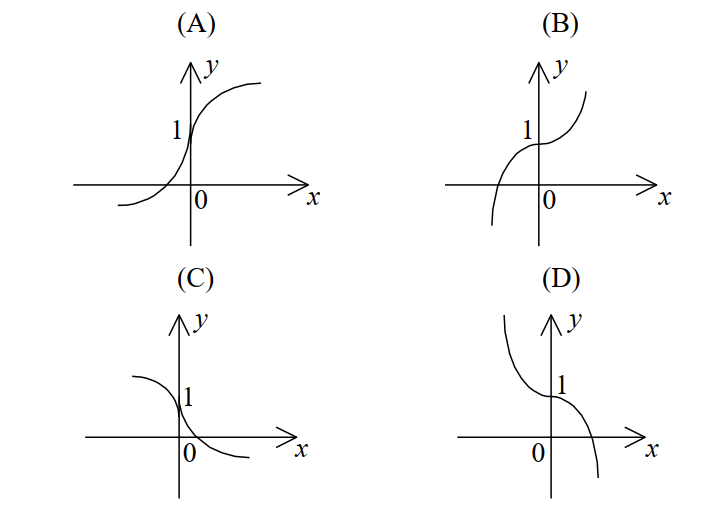
\includegraphics{D:/sslchi.github.io/calculus/HW_chap4a.png}
%		\caption{HW\_chap1a}
%	\end{figure}


\kpoint{曲线的凸凹性与拐点}
\end{problem}
\begin{problem}
设 $\displaystyle f\left( x \right) = \frac{\ln x}{x}$, 则使不等式
$\displaystyle \frac{\ln a}{a} > \frac{\ln b}{b}$ 成立的条件是\pickin{B}.

\begin{abcd} 
	
	\item $\ 0 < a < b;$
	
	\item $\e < a < b;$
	
	\item $\ 0 < b < a;$
	
	\item $\e < b < a.$

\end{abcd}

\kpoint{函数单调性的判别法}
\end{problem}

\begin{problem}
关于函数 $y = x - \ln x$ 的极值, 结论正确的是\pickin{A}.

\begin{abcd} 
\item 有极小值 $1$;

\item 有极大值 $1$;

\item 无极值 $\e - 1$;

\item 有极小值 $\e - 1$.

\end{abcd}

\kpoint{函数极值的第一充分条件}
\end{problem}

\begin{problem}
关于函数 $y = 2x - {\ln\left( 4x \right)}^{2}$ 的极值,
结论正确的是\pickin{B}.

\begin{abcd} \item 有极大值 $2 - 4\ln 2;$

\item 有极小值 $2 - 4\ln 2;$

\item 无极值;

\item 有极小值 $\frac{1}{2}.$

\end{abcd}


\kpoint{函数极值的第一充分条件}
\end{problem}

\begin{problem}
曲线 $y = 3x^{2} - x^{3}$ 在\pickin{B}

\begin{abcd} 
\item $\left( 1, + \infty \right)$是凹的, $\left( - \infty,1 \right)$
是凸的;

\item $\left( 1, + \infty \right)$是凸的, $\left( - \infty,1 \right)$
是凹的;

\item $\left( 0, + \infty \right)$内是凸的,
在$\left( - \infty,0 \right)$是上凹的;

\item $\left( 0, + \infty \right)$ 内是上凹的,
$\left( - \infty,0 \right)$ 是上凸的;

\end{abcd} 

\kpoint{曲线的凸凹性判别}
\end{problem}

\begin{problem}
曲线 $y = x^{2}\ln x$ 在点
$\displaystyle \left( \frac{1}{\e^{4}},\frac{1}{\e^{2}} \right)$ 近邻是\pickin{A}.

\begin{abcd} \item 向上凸的; \item 向上凹的;

\item 左侧近邻向上凸, 右侧近邻向上凹;

\item 左侧近邻向上凹, 右侧的邻向上凸;

\end{abcd}

\kpoint{曲线的凸凹性判别}
\end{problem}

\begin{problem}
曲线 $y = \e^{- x^{2}}$ 的拐点情况是\pickin{C}.

\begin{abcd} \item 没有拐点;

\item 有一个拐点;

\item 有两个拐点;

\item 有三个拐点.

\end{abcd}

\kpoint{曲线的凸凹性与拐点}

\end{problem}

\begin{problem}
若 $\left( x_{0},f\left( x_{0} \right) \right)$ 为连续曲线
$y = f\left( x \right)$ 上的凹弧与凸弧分界点, 则\pickin{A}.

\begin{abcd} \item $\left( x_{0},f\left( x_{0} \right) \right)$ 必为曲线的拐点;

\item $\left( x_{0},f\left( x_{0} \right) \right)$ 必定为曲线的驻点;

\item $x_{0}$ 为 $f\left( x \right)$ 的极值点;

\item $x_{0}$ 必定不是 $f\left( x \right)$ 的极值点;

\end{abcd}

\kpoint{曲线的凸凹性与拐点}
\end{problem}


\begin{problem}
曲线 $\left\{ \begin{matrix}
 x = a(t - \sin t) \\
 y = a(1 - \cos t) \\
\end{matrix}(a > 0) \right.\ $\pickin{C}.

\begin{abcd} \item 有无穷多个拐点;

\item 有两个拐点;

\item 无拐点;

\item 有一个拐点.

\end{abcd}

\kpoint{曲线的凸凹性与拐点}
\end{problem}


\begin{problem} 
点 $(0,1)$ 是曲线 $y = ax^{3} + bx^{2} + c$ 的拐点, 则必有\pickin{B}.

\begin{abcd} \item $a = 1,\ b = - 3,\ c = 1;$

\item $a$ 任意, $b = 0,\ c = 1;$

\item $a = 1,\ b = 0,$ $c$ 任意;

\item $b = - 3a$, $a$ 任意, $c = 1$.

\end{abcd}

\kpoint{曲线的凸凹性与拐点}
\end{problem}

\begin{problem}
关于曲线 $y = \ln x$ 的渐近线, 下述结论正确的是\pickin{B}.

\begin{abcd} \item 只有水平渐近线;

\item 只有铅直渐近线;

\item 既有水平渐近线, 又有铅直渐近线 ;

\item 既没有水平渐近线, 也没有铅直渐近线.

\end{abcd}

\kpoint{曲线的渐近线}
\end{problem}

\begin{problem}
$\displaystyle \lim\limits_{x \rightarrow \frac{\pi}{2}}\left( \frac{\cos 5x}{\cos 3x} \right)$=
\pickin{A}

\begin{abcd} \item $- 5/3;$

\item $- 1;$

\item $1;$

\item $5/3.$

\end{abcd}

\kpoint{洛必达法则}
\end{problem}

\begin{problem}
在区间 $\lbrack 0,8\rbrack$ 内, 对函数
$f\left( x \right) = \sqrt[3]{8x - x^{2}}$, 罗尔定理\pickin{C}.

\begin{abcd} \item 不成立;

\item 成立, 并且 $f'\left( 2 \right) = 0;$

\item 成立, 并且 $f'\left( 4 \right) = 0;$

\item 成立, 并且 $f'\left( 8 \right) = 0$.

\end{abcd}

\kpoint{罗尔定理}
\end{problem}

\begin{problem}
设 $f(x)\ $ 在 $\left\lbrack a,b \right\rbrack$ 上连续, 在
$\left( a,b \right)$ 内可导, 记(I)
$f\left( a \right) = f\left( b \right)$; (II) 在 $\left( a,b \right)$
内至少存在 $\xi$, 使 $f'\left( \xi \right) = 0$, 则\pickin{A}.

\begin{abcd} \item(I)是(II) 的充分但非必要条件;

\item(I)是(II) 的必要但非充分条件;

\item (I) 是(II) 的充要条件;

\item (I) 是(II) 既非充分, 也非必要条件.

\end{abcd}

\kpoint{罗尔定理}
\end{problem}

\begin{problem}
设 $f(x) = \left\{ \begin{matrix}
3 - x^{2},\ \ \ \ 0 \leq |x| \leq 1 \\
\displaystyle \frac{2}{x},\ \ \ \ 1 < |x| \leq 2 \\
\end{matrix}\ \ , \right.\ $ 则在区间内 $(0,2)$ 满足
$f\left( 2 \right) - f\left( 0 \right) = f'\left( \xi \right)\left( 2 - 0 \right)$
的 $\xi$ 值\pickin{C}.

\begin{abcd} \item 只有一个;

\item 不存在;

\item 有两个;

\item 有三个.

\end{abcd}

\kpoint{拉格朗日中值定理}
\end{problem}

\begin{problem}
设 $a < b,ab < 0,f\left( x \right) =\displaystyle  \frac{1}{x}$, 则在
$a < x < b$ 内使
$f\left( b \right) - f\left( a \right) = f'\left( \xi \right)\left( b - a \right)$
成立的点 $\xi$ \pickin{C}.

\begin{abcd} \item 只有一点;

\item 有两点;

\item 不存在;

\item 是否存在,与 $a,b\ $ 的具体数值有关.

\end{abcd}

\kpoint{拉格朗日中值定理}
\end{problem}

\begin{problem}
设 $f(x)$ 有直至 $n + 1$ 阶导数, 则
$\displaystyle f\left( x \right) = \sum_{k = 1}^{n}{\frac{f^{\left( k \right)}\left( 0 \right)}{k!}x^{k}} + R_{n}\left( x \right)$式中拉格朗日型余项
$R_{n}\left( x \right)$ =\pickin{B}(设 $0 < \theta < 1$)

\begin{abcd} \item $\displaystyle \frac{f^{\left( n \right)}\left( \theta x \right)}{n!}x^{n};$

\item
$\displaystyle \frac{f^{\left( n + 1 \right)}\left( \theta x \right)}{\left( n + 1 \right)!}x^{n + 1};$

\item
$\displaystyle \frac{f^{\left( n + 1 \right)}\left( x \right)}{\left( n + 1 \right)!}\left( \theta x \right)^{n + 1};$

\item
$\displaystyle \frac{f^{\left( n + 1 \right)}\left( \theta \right)}{\left( n + 1 \right)!}x^{n + 1}$.

\end{abcd}

\kpoint{泰勒公式(大纲无此内容)}
\end{problem}

\begin{problem}
已知函数 $f\left( x \right) = x^{3} + ax^{2} + bx$ 在点 $x = 1$
处取得极值 $- 2$, 则\pickin{B}.

\begin{abcd}

\item $a = - 3,\ b = 0$ 且点 $\ x = 1\ $为函数 $f(x)$ 的极小值;

\item $a = 0,\ b = - 3$ 且点 $x = 1$ 为函数 $f(x)$ 的极小值;

\item $a = - 3,\ b = 0$ 且点 $x = 1$ 为函数 $f(x)$ 的极大值;

\item $a = 0,\ b = - 3\ $ 且点 $x = 1\ $为函数 $f(x)$ 的极大值.

\end{abcd}

\kpoint{函数极值的第一充分条件}
\end{problem}

\begin{problem} 
函数
$f\left( x \right) = \displaystyle \frac{\sqrt{x - 1}}{x\left( x - 1 \right)\left( x - 2 \right)}$
的所有渐近线有\pickin{B}条

\begin{abcd} \item $4;$

\item $3;$

\item $2;$

\item $1$.

\end{abcd}

\kpoint{曲线的渐近线}
\end{problem}

\makepart{填空题}

\begin{problem} 曲线 $y = 1 - \sqrt[3]{x - 2}$ 的拐点是\fillin{$(2,1)$}.

\kpoint{曲线的凸凹性与拐点}
\end{problem}

\begin{problem} 设函数 $f(x)$ 在 $(a,b)$ 内可导且满足
$f'\left( x \right) \equiv 0$, 则在 $(a,b)$ 内 $f(x)\ $=
\fillin{ $C,\ C$ 为常数}.

\kpoint{拉格朗日中值定理}
\end{problem}

\begin{problem} 设函数 $f(x)$ 在 $x = 0$ 处具有二阶导数, 且 $f(0) = 0,$
$f'\left( 0 \right) = 1,$ $f''\left( 0 \right) = 3,$ 则极限
$\displaystyle \lim\limits_{x \rightarrow 0}\frac{f\left( x \right) - x}{x^{2}}$ =\fillin{ $\displaystyle \frac{3}{2}$}.

\kpoint{洛必达法则}
\end{problem}

\begin{problem} $\displaystyle \lim\limits_{x \rightarrow 0}\frac{\ln{\cos a}x}{\ln{\cos b}x}$
的值等于\fillin{$\displaystyle \frac{a^{2}}{b^{2}}.$}, $\left( b \neq 0 \right).$.



\kpoint{洛必达法则}
\end{problem}


\begin{problem} 设 $a > 0,$ 则
$\lim\limits_{x \rightarrow + \infty}\displaystyle \frac{\ln x}{\e^{{ax}}}$
的值等于\fillin{ $0$}.

\kpoint{洛必达法则}
\end{problem}

\begin{problem} $f\left( x \right) = x^{3}$
在$\lbrack 0,1\rbrack$上满足拉格朗日中值定理的 $\xi$
=\fillin{ $\displaystyle \frac{\sqrt{3}}{3}$}.

\kpoint{拉格朗日中值定理}
\end{problem}

\begin{problem} 函数 $f\left( x \right) = 1 - \sqrt[3]{x^{2}}$ 在
$\lbrack - 1,\ 1\rbrack$ 上不具有罗尔定理的结论, 其原因是由于 $f(x)$
不满足罗尔定理的一个条件\fillin{ $f(x)$ 在 $\left( - 1,1 \right)$ 内可导}.

\kpoint{罗尔定理}
\end{problem}

\begin{problem} $\lim\limits_{x \rightarrow 0}\displaystyle \frac{3x - \sin 3x}{x^{3}}$ 的值等于
\fillin{ $\displaystyle \frac{9}{2}$}.

\kpoint{洛必达法则}
\end{problem}

\begin{problem} $\lim\limits_{x \rightarrow + \infty}\displaystyle \frac{\e^{x}}{x^{a}}$ = \fillin{$+ \infty$}
($a > 0$).



\kpoint{洛必达法则}
\end{problem}

\begin{problem} $\lim\limits_{x \rightarrow \pi}\displaystyle \frac{\e^{\pi} - \e^{x}}{\sin 3x - \sin x}$
的值等于\fillin{ $\displaystyle \frac{1}{2}\e^{\pi}$}.

\kpoint{洛必达法则}
\end{problem}

\begin{problem} $\lim\limits_{x \rightarrow 0}\displaystyle \frac{\e^{3x} - 1 - x}{2x}$
的值等于\fillin{$1$}.

\kpoint{洛必达法则}
\end{problem}

\begin{problem} $\lim\limits_{x \rightarrow 0}\displaystyle \frac{\e^{x^{2}} - \cos x}{x^{2}}$
的值等于\fillin{ $\displaystyle \frac{3}{2}$}.


\kpoint{洛必达法则}
\end{problem}

\begin{problem} $\lim\limits_{x \rightarrow 0}\displaystyle \frac{x - \ln\left( 1 + x \right)}{x^{2}}$
的值等于\fillin{ $\displaystyle \frac{1}{2}$}.

\kpoint{洛必达法则}
\end{problem}

\begin{problem} $\lim\limits_{x \rightarrow \pi}\displaystyle \frac{\tan nx}{\tan mx}$( 其中 $m,\ n$
为正整数) 的值等于\fillin{ $\displaystyle \frac{n}{m}$}.

\kpoint{洛必达法则}
\end{problem}

\begin{problem} $\displaystyle \lim\limits_{x \rightarrow 0}\frac{x}{\e^{x} - \e^{- x}}$
的值等于\fillin{ $\displaystyle \frac{1}{2}$}.

\kpoint{洛必达法则}
\end{problem}

\begin{problem} $\displaystyle \lim\limits_{x \rightarrow + \infty}\frac{x^{k}}{\e^{x}}$( 其中
$k > 0$) 的值等于\fillin{ $0$}.

\kpoint{洛必达法则}
\end{problem}

\begin{problem} $\displaystyle {\lim\limits_{x \rightarrow + \infty}\left( \ln x \right)}^{1/x}$
= \fillin{ $1$}.

\kpoint{洛必达法则}
\end{problem}

\begin{problem}
$\displaystyle \lim\limits_{h \rightarrow 0}\frac{\ln\left( x + h \right) + \ln\left( x - h \right) - 2\ln x}{h^{2}}$
= \fillin{$\displaystyle - \frac{1}{x^{2}}$}.

\kpoint{洛必达法则}
\end{problem}

\begin{problem} 曲线 $\displaystyle y = \frac{x^{2}}{2x + 1}$ 的斜渐近线为
\fillin{ $\displaystyle y = \frac{1}{2}x - \frac{1}{4}$}.

\kpoint{曲线的渐近线}
\end{problem}

\begin{problem}
曲线 $\displaystyle y = \frac{\e^{x}}{x + 1}$ 有\fillin{零}个拐点.



\kpoint{曲线的凸凹性与拐点}
\end{problem}

\makepart{计算题}

\begin{problem} 判定函数
$f\left( x \right) = x + \cos x\left( 0 \leq x \leq 2\pi \right)$
的单调性.

\begin{solution}
由条件知:$$f'\left( x \right) = 1 - \sin x \geq 0,x \in \left\lbrack 0,2\pi \right\rbrack,$$
且在 $\left( 0,2\pi \right)$ 内使
$f'\left( x \right) = 1 - \sin x = 0$ 的点 $\displaystyle x = \frac{\pi}{2}$
是孤立的.故 $f\left( 0 \right) = x + \cos x$ 在区间
$\left\lbrack 0,2\pi \right\rbrack$ 上单调增加.

\end{solution}
\kpoint{函数单调性的判别法}
\end{problem}

\begin{problem} 求函数 $y = \left( x + 1 \right)^{4} + \e^{x}$
的图形的抛点及凹凸区间.

\begin{solution} 函数的定义域为 $R$, $y' = 4\left( x + 1 \right)^{3} + \e^{x}$,
因为
$$y'' = 12\left( x + 1 \right)^{2} + \e^{x} > 0$$

所以 $y$ 在 $R$ 上都是凹的, 无拐点.

\end{solution}
\kpoint{曲线的凸凹性与拐点}
\end{problem}

\begin{problem} 求极限
$\displaystyle \lim\limits_{x \rightarrow \frac{\pi}{4}}\frac{\cos 2x}{\e^{\sin 4x} - \e^{\sin 8x}}$.

\begin{solution} 原式等于
$$\lim\limits_{x \rightarrow \frac{\pi}{4}}\frac{- 2\sin 2x}{\e^{\sin 4x} \cdot 4\cos 4x - 8\e^{8\sin x} \cdot \cos 8x} = \frac{1}{6}.$$

\end{solution}
\kpoint{洛必达法则}
\end{problem}

\begin{problem} 设 $f(x)$ 有一阶导数,
$f\left( 0 \right) = f'\left( 0 \right) = 1$, 求
$\displaystyle \lim\limits_{x \rightarrow 0}\frac{f\left( \sin x \right) - 1}{\ln f\left( x \right)}$

\begin{solution} 有洛必达法则可知
$$\lim\limits_{x \rightarrow 0}\frac{f\left( \sin x \right) - 1}{\ln f\left( x \right)} = \lim\limits_{x \rightarrow 0}\frac{f'\left( \sin x \right) \cdot \cos x}{f'\left( x \right)\text{/}f\left( x \right)} = \frac{f'\left( 0 \right) \cdot \cos 0}{f'\left( 0 \right)\text{/}f\left( 0 \right)} = 1.$$

\end{solution}\kpoint{洛必达法则}
\end{problem}

\begin{problem} 求极限
$\displaystyle \lim\limits_{x \rightarrow 0}\frac{12^{x} - 5^{- 3x}}{ 2\arcsin x - x}$

\begin{solution} 原式等于
$$\lim\limits_{x \rightarrow 0}\frac{12^{x}\ln 12 + 3 \cdot 5^{- 3x}\ln 5}{2 \cdot \displaystyle \frac{1}{\sqrt{1 - x^{2}}} - 1} = \ln 12 + 3\ln 5.$$

\end{solution}\kpoint{洛必达法则}
\end{problem}

\begin{problem} 求极限
$$\lim\limits_{x \rightarrow 1}\frac{\tan{\ln\left( 3x - 2 \right)}}{\e^{x + 1} - \e^{x^{2} + 1}}$$

\begin{solution} 原式等于

$$\lim\limits_{x \rightarrow 1}\frac{\sec^{2}{\ln\left( 3x - 2 \right)} \cdot \displaystyle \frac{3}{3x - 2}}{\displaystyle \e^{x + 1} - 2x\e^{x^{2} + 1}} = - \frac{3}{\e^{2}}.$$

\end{solution}
\kpoint{洛必达法则}
\end{problem}

\begin{problem} 求极限
$\displaystyle \lim\limits_{x \rightarrow 0}\frac{\ln\left| \sin ax \right|}{\ln\left| \sin bx \right|}$
( $a,b$ 都是不为 $0$ 的常数).

\begin{solution} 原式等于
$$\lim\limits_{x \rightarrow 0} \dfrac{\frac{a\cos ax}{\sin ax}}{\frac{b\cos x}{\sin bx}} = \lim\limits_{x \rightarrow 0}\frac{{ax}}{\sin ax} \cdot \frac{\sin bx}{\text{bx}} \cdot \frac{\cos ax}{\cos bx} = 1.$$

\end{solution}
\kpoint{洛必达法则}
\end{problem}

\begin{problem} 试决定曲线 $y = ax^{3} + bx^{2} + cx + d$ 中的 $a,\ b,\ c,\ d,$
使得 $x = - 2$ 处曲线有水平切线, $(1, - 10)$ 为拐点, 且点
$( - 2,\ 44)$ 在曲线上.

\begin{solution} 由题设可知, 驻点与拐点都在曲线上, 从而有
\begin{eqnarray}
- 8a + 4b - 2c + d = 44,\label{eq:1}\\
a + b + c + d = - 10,\label{eq:2}\\
y' = 3ax^{2} + 2bx + c,\notag\\
y'' = 6ax + 2b.\notag
\end{eqnarray}

由驻点和拐点的条件可得
\begin{eqnarray}
12a - 4b + c = 0,\label{eq:3}\\
6a + 2b = 0.\label{eq:4}
\end{eqnarray}

联立\eqref{eq:1}-\eqref{eq:4}解得
$$a = 1,\ b = - 3,\ c = - 24,\ d = 16.$$

\end{solution}
\kpoint{曲线的凸凹性与拐点}

\end{problem}

\begin{problem} 求函数 $y = x^{5} - 5x^{4} + 5x^{3} + 1$ 在
$\lbrack - 1,2\rbrack$ 上的最大值, 最小值.

\begin{solution} 由条件可得:
$$y' = 5x^{2}\left( x - 1 \right)\left( x - 3 \right)$$

函数在 $\lbrack - 1,2\rbrack$ 上的驻点为: $x_{1} = 0,x_{2} = 1$, 而
\begin{eqnarray}
y\left( 0 \right) = 1,y\left( 1 \right) = 2,\\
y\left( - 1 \right) = - 10,y\left( 2 \right) = - 7.
\end{eqnarray}

所以
$$y_{\max} = y\left( 1 \right) = 2,y_{\min} = y\left( - 1 \right) = - 10.$$

\end{solution}\kpoint{函数的最大值与最小值

}\end{problem}

\begin{problem} 求曲线 $\displaystyle y = \frac{\e^{x}}{1 + x}$ 的渐近线

\begin{solution} 因为
$$\lim\limits_{x \rightarrow - 1}\frac{\e^{x}}{1 + x} = \infty,\ \lim\limits_{x \rightarrow - \infty}\frac{\e^{x}}{1 + x} = \lim_{x \rightarrow - \infty}\frac{1}{1 + x} \cdot \frac{1}{\e^{- x}} = 0.$$

所以 $x = - 1$ 是垂直渐近线, $y = 0$ 是水平渐近线.

\end{solution}
\kpoint{曲线的渐近线}
\end{problem}



\makepart{综合与应用题}


 \begin{problem} 用长度为 $l$ 米( $\ l > 0$
)的篱笆在直的河岸边围成三面是篱笆一面是河的矩形场地,
求矩形场地的最大面积.

%	\begin{figure}
%		\centering
%		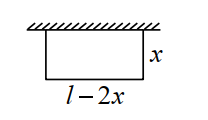
\includegraphics{D:/sslchi.github.io/calculus/HW_chap4b.png}
%		\caption{}
%	\end{figure}

\begin{solution}如图, 设靠河的篱笆长为 $x$, 则矩形场地的面积为
$$S = x(l - 2x),$$则
$$S' = l - 4 x$$, 得唯一驻点 $\displaystyle x = \frac{l}{4}$.
显然存在最大面积, 所以
$$S_{\max} = S\left( \frac{l}{4} \right) = \frac{l^{2}}{8}.$$
\end{solution}

\kpoint{函数最值的应用}

\end{problem}        

  
\begin{problem} 要做一个圆锥形漏斗, 其母线长 20 cm, 要使其体积最大, 问其高应为多少?

\begin{solution} 设圆锥形漏斗的高为 $H$cm, 则圆锥底面半径为
$$R = \sqrt{400 - H^{2}}$$
漏斗的体积为
$$V = \frac{\pi}{3}\left( 400 - H^{2} \right)H,\ 0 < H < 20,$$

又因为
$$V' = \frac{\pi}{3}\left( 400 - 3H^{2} \right),$$

所以体积函数 $V$ 在$(0, 20)$内有唯一驻点
$$H = \frac{20\sqrt{3}}{3},$$

又因为
$$V'' = - 2\pi H < 0,$$

因此唯一驻点 $\displaystyle H = \frac{20\sqrt{3}}{3}$ 也是极大值点, 由实际问题可知,
此时漏斗体积最大.
\end{solution}
\kpoint{函数最值的应用}

\end{problem}           

\begin{problem} 设有一块边长为 $a$ 的正方形铁皮, 从四个角截去同样的小方块,
做成一个无盖的方盒子, 问小方块的边长为多少才使盒子的容积最大?

\begin{solution} 设小方块的边长为 $x$, 则盒子的容积为
$$V = x\left( a - 2x \right)^{2} = a^{2}x + 4x^{3} - 4ax^{2},\quad 0 < x < \frac{a}{2},$$

其导数为
$$V' = a^{2} + 12x^{2} - 8ax$$

唯一驻点 $\displaystyle x = \frac{a}{6}$. 又
$$\left. \ V'' \right|_{x = \frac{a}{6}} = \left. \ \left( 24x - 8a \right) \right|_{x = \frac{a}{6}} = - 4a < 0,$$

即 $\displaystyle x = \frac{a}{6}$ 为极大值点, 也是最大值, 所以小方块边长为
$\displaystyle \frac{a}{6}$ 时, 盒子的容积最大.
\end{solution}
\kpoint{函数最值的应用}

\end{problem}           

\begin{problem} 设某产品的销售量 $Q$ 与价格 $P$ 之间有关系式为
$\displaystyle Q = \frac{1 - P}{P}$

(1) 求需求弹性 ;

(2) 售价为 $0.5$ 时的需求弹性. 并给出经济解释.

\begin{solution}(1)
$$\eta = - Q'\left( P \right)\frac{P}{Q\left( P \right)} = \frac{1}{P^{2}}\frac{P}{\frac{1 - P}{P}} = \frac{1}{1 - P}$$

(2)
$$\eta\left( 0.5 \right) = \left. \ \frac{1}{1 - P} \right|_{P = 0.5} = 2$$

其经济意义为: 在售价为 $0.5$ 时的水平上, 若价格上涨 $1\%$,
需求量下降 $2\%.$
\end{solution}
\kpoint{弹性(应该放在第三章)}

\end{problem}           

\begin{problem} 某厂生产某种商品, 其年销售量为 $100$ 万件,
每批生产需增加准备费1000元, 而每件的库存费为0.05元. 如果年销售是均匀的,
且上批销售完后, 立即再生产下一批(此时商品库存量为批量的一半),
问分几批生产, 能使生产准备费及库存费之和最小?

\begin{solution} 设每批生产 $x$ 件, 则有
$$y = 1000 \times \frac{1000000}{x} - \frac{x}{2} \times 0.05,$$
其导数为:
$$y' = \frac{10^{9}}{x^{2}} - 0.025$$

令 $y' = 0$, 得 $x = 200000$ (件)(舍去负根).
$$y'' = \frac{2 \times 10^{9}}{x^{3}},\ y''\left( 200000 \right) > 0,$$

即批量 $200000$(件), 批次为 $5$ 时总费用最小.
\end{solution}
\kpoint{函数最值的应用}

\end{problem}           

\begin{problem} 某商品的价格 $P$ 与需求量 $Q$ 的关系为 $\displaystyle P = 10 - \frac{Q}{5}$,

(1) 求需求量为 $20$ 及 $30$ 时的总收益 $R$、平均收益
$\overline{R}$ 及边际收益 $R'$;

(2) $Q$ 为多少时总收益最大?

\begin{solution}
由条件知
$$R = R\left( Q \right) = QP\left( Q \right) = 10Q - \frac{Q^{2}}{5}$$
$$\overline{R}\left( Q \right) = P\left( Q \right)$$
$$R'\left( Q \right) = 10 - \frac{2Q}{5}$$

(1)由条件知:
$$R\left( 20 \right) = 120,R\left( 30 \right) = 120,\overline{R}\left( 20 \right) = 6,$$
$$\overline{R}\left( 30 \right) = 4,R'\left( 20 \right) = 2,R'\left( 30 \right) = - 2.$$

(2) 令 $R'\left( Q \right) = 0$, 得 $Q = 25$, 又
$$R''\left( Q \right) = - \frac{2}{5} < 0,$$ 所以 $Q = 25$
时总收益最大.
\end{solution}
\kpoint{函数最值的应用}

\end{problem}           

\begin{problem} 设 $f\left( x \right) = x^{3} + ax^{2} + bx$ 在 $x = 1$ 处有极值
$- 2$, 试确定系数 $a,\ b,$ 并求出 $y = f\left( x \right)$
的所有极值点及拐点.

\begin{solution} 由题意知
$$f'\left( x \right) = 3x^{2} + 2ax + b$$

由于 $f\left( x \right)$ 在点 $x = 1$ 有极值 $- 2$, 所以
$$f\left( 1 \right) = 1 + a + b = - 2,\ f'\left( 1 \right) = 3 + 2a + b = 0 \Rightarrow a = 0,b = - 3,$$

因此
$$f\left( x \right) = x^{3} - 3x,f'\left( x \right) = 3x^{2} - 3,f''\left( x \right) = 6x.$$

所以极值点为 $x = 1$ 和 $x = - 1,$ 拐点为 $(0, 0).$
\end{solution}
\kpoint{函数极值的第二充分条件}

\end{problem}           

\begin{problem} 在半径为 $R$ 的球内, 求体积最大的内接圆柱体的高.

\begin{solution} 设内接圆柱体的高为 $h$ , 则圆柱体的底面半径
$$r = \sqrt{R^{2} - \left( \frac{h}{2} \right)^{2}},$$

其体积为
$$V = \pi h\left( R^{2} - \frac{h^{2}}{4} \right),\quad 0 < h < 2R,$$

其导函数为
$$V' = \pi\left( R^{2} - \frac{3}{4}h^{2} \right)$$

故其有唯一驻点
$$h = \frac{2\sqrt{3}}{3}R,$$

又因为
$$V'' = - \frac{3}{2}\pi h < 0,$$

故 $\displaystyle h = \frac{2\sqrt{3}}{3}R$ 时, 圆柱体体积最大.
\end{solution}
\kpoint{函数最值的应用}

\end{problem}           

\begin{problem} 由三块同一宽度的板做成一个梯形的排水槽(无上盖), 问侧面与底的倾角
$\alpha$ 为多大时, 才使水槽的横断面积最大?

\begin{solution} 设板宽为 $a$, 侧面与底面的倾角为 $\alpha$ 则横断面面积为
$$S = \frac{1}{2}\left( 2a + 2a\cos\alpha \right)a\sin\alpha = a^{2}\left( 1 + \cos\alpha \right)\sin\alpha,\ \  0 < \alpha < \frac{\pi}{2}.$$

其导数为
$$S' = a^{2}\left( 2\cos^{2}\alpha + \cos\alpha - 1 \right)$$

该函数的唯一驻点 $\alpha = \frac{\pi}{3}$.

又因为
$$S'' = - a^{2}\left( 2\sin 2\alpha + \sin\alpha \right),\left. \ \quad S'' \right|_{\alpha = \frac{\pi}{3}} = - \frac{3\sqrt{3}}{2}a^{2} < 0$$

所以当 $\displaystyle \alpha = \frac{\pi}{3}$ 时, 横断面面积最大.
\end{solution}
\kpoint{函数最值的应用}

\end{problem}           


\begin{problem} 将半径为 $r$ 的圆铁片, 剪去一个扇形, 问其中心角 $\alpha$
为多大时, 才能使余下部分围成的圆锥形容器的容积最大?

\begin{solution} 设圆雉形容器半径为 $R$, 高为 $h$, 容积为 $V$, 则
$$R^{2} + h^{2} = r^{2},V = \frac{1}{3}\pi R^{2}h = \frac{\pi}{3}\left( r^{2} - h^{2} \right)h$$

令
$$\frac{\text{d}V}{\text{d}h} = \frac{\pi}{3}\left( r^{2} - 3h^{2} \right) = 0,$$
求得的唯一驻点为 $$h = \frac{r}{\sqrt{3}},$$ 此时
$\displaystyle R = \frac{\sqrt{2}}{\sqrt{3}}\text{r.}$ 依问题的实际意义, $V$
存在最大值.故 $\displaystyle R = \frac{\sqrt{2}}{\sqrt{3}}r$ 为所求 , 但
$$2\pi R = \left( 2\pi - \alpha \right)r,$$ 解得
$$\alpha = \left( 1 - \frac{\sqrt{6}}{3} \right) \cdot 2.$$ 即
$$\alpha = 1 - \frac{\sqrt{6}}{3} \cdot 2$$ 时所求容积最大.
\end{solution}
\kpoint{函数最值的应用}

\end{problem}

\makepart{证明题}



\begin{problem} 设 $f\left( x \right)$ 在 $\left\lbrack 1,\e \right\rbrack$
上连续, 在 $(1,\e)$ 内可导, 且
$f\left( 1 \right) = 0,f\left( \e \right) = 1,$ 证明方程
$xf'\left( x \right) = 1$ 在 $\left( 1,\e \right)$ 内至少有一实根.

\begin{solution}
证明: 令 $F\left( x \right) = f\left( x \right) - \ln x,$ 则
$F\left( x \right)$ 在 $\left\lbrack 1,\e \right\rbrack$ 上连续, 在
$(1,\e)$ 内可导. {因}
$f\left( 1 \right) = 0,f\left( \e \right) = 1,$ {则}
$F\left( 1 \right) = F\left( \e \right) = 0,$ {即}
$F\left( x \right)$ {在} $\left\lbrack 1,\e \right\rbrack$
{上满足罗尔定理的条件, 则至少存在}
$\xi \in \left( 1,\e \right)${, 使} $F'\left( \xi \right) = 0,$
而
$$F'\left( x \right) = f'\left( x \right) - \frac{1}{x},$$
即
$$f'\left( \xi \right) - \frac{1}{\xi} = 0,\quad\xi \in \left( 1,\e \right)$$
即
$$\xi f'\left( \xi \right) = 1.$$
故 $xf'\left( x \right) = 1$ 在 $(1,\e)$ 内至少有一个实根.

\end{solution}

\kpoint{罗尔定理}


\end{problem}           


\begin{problem} 设 $f\left( x \right)$ 在 $\left\lbrack a,b \right\rbrack$
上可导, 证明存在 $\xi \in \left( a,b \right),$ 使
$$\frac{1}{b - a}\left| \begin{matrix}
b^{3} & a^{3} \\
f\left( a \right) & f\left( b \right) \\
\end{matrix} \right| = \xi^{2}\left\lbrack 3 f\left( \xi \right) + \xi f'\left( \xi \right) \right\rbrack.$$

\begin{solution}
	证明: 令 $F\left( x \right) = x^{3}f\left( x \right),$ 则
$F\left( x \right)$ 在 $\left\lbrack a,b \right\rbrack$ 上可导,
利用拉格朗日中值定理, 则至少存在 $\xi \in \left( a,b \right),$ 使
$$F\left( b \right) - F\left( a \right) = F'\left( \xi \right)\left( b - a \right),$$
即
$$b^{3}f\left( b \right) - a^{3}f\left( a \right) = \left\lbrack 3\xi^{2}f\left( \xi \right) + \xi^{3}f'\left( \xi \right) \right\rbrack\left( b - a \right),$$
即
$$\frac{1}{b - a}\left| \begin{matrix}
b^{3} & a^{3} \\
f\left( a \right) & f\left( b \right) \\
\end{matrix} \right| = \xi^{2}\left\lbrack 3 f\left( \xi \right) + \xi f'\left( \xi \right) \right\rbrack.$$
\end{solution}

\kpoint{拉格朗日中值定理}
\end{problem} 

\begin{problem}
设 $f\left( x \right)$ {在}
$\left\lbrack 1,2 \right\rbrack$ {上连续, 在} $(1,\ 2)$
{内可导, 且} $f\left( 2 \right) = 0,$ {证明至少存在一点}
$\xi \in \left( 1,2 \right),$ {使}
$$f'\left( \xi \right) = - \frac{f\left( \xi \right)}{\xi\ln\left( \xi \right)}.$$

\begin{solution}
{证明: 令} $F\left( x \right) = f\left( x \right)\ln x${,
	则} $F\left( x \right)$ {在} $\lbrack 1,\ 2\rbrack$
{上连续, 在} $(1,\ 2)$ {内可导, 且}
$$F\left( 1 \right) = f\left( 1 \right)\ln 1 = 0,\quad F\left( 2 \right) = f\left( 2 \right)\ln 2 = 0.$$

{即} $F\left( x \right)$ {在} $\lbrack 1,2\rbrack$
{上满足罗尔定理的条件, 则至少存在}
$\xi \in \left( 1, 2 \right)$ {使}
$F'\left( \xi \right) = 0,$ {而}
$$F'\left( x \right) = f'\left( x \right)\ln x + f\left( x \right) \cdot \frac{1}{x}$$
{即有}
$$f'\left( \xi \right) = - \frac{f\left( \xi \right)}{\xi\ln\left( \xi \right)}.$$

\end{solution}
\kpoint{罗尔定理}

\end{problem}           

\begin{problem} 设 $b > a > 0,$ {证明 :}
$\displaystyle \ln\frac{b}{a} > \frac{2\left( b - a \right)}{a + b}.$

\begin{solution}
证明: 令
$f\left( x \right) = \left( a + x \right)\left( \ln x - \ln a \right) - 2\left( x - a \right),$则
$$f\left( a \right) = 0,f'\left( x \right) = \ln x–\ln a + \left( a + x \right)\frac{1}{x} - 2,$$
{即}
$$f'\left( x \right) = \ln x - \ln a + \frac{a}{x} - 1$$
{故} $f'\left( a \right) = 0.$ {又因为}
$$f''\left( x \right) = \frac{1}{x} - \frac{a}{x^{2}} = \frac{x - a}{x^{2}} > 0\quad\left( x > a \right),$$
{所以} $f''\left( x \right)$ {单调递增,}
$f'\left( x \right) > f\left( a \right) = 0,$ {所以函数}
$f\left( x \right)$ {单调递增, 于是当} $x > a$ {时}
$f\left( x \right) > f\left( a \right) = 0,$ {令}
$x = b${, 则} $f\left( b \right) > f\left( a \right) = 0,$
{即}
$$\left( a + b \right)\left( \ln b - \ln a \right) - 2\left( b - a \right) > 0,$$
{亦即}
$$\ln\frac{b}{a} > \frac{2\left( b - a \right)}{a + b}.$$
\end{solution}
\kpoint{ 函数单调性的判别法}

\end{problem}           

\begin{problem} 证明当 $x \neq 0$ {时, 有不等式} $\e^{x} > 1 + x.$

\begin{solution}
证明:令 $$f\left( x \right) = \e^{x} - x - 1,$$
它在
$\left( - \infty, + \infty \right)$ 连续.易知
$$f'\left( x \right) = \e^{x} - 1,\ f''\left( x \right) = \e^{x} > 0.\
f'\left( 0 \right) = 0,f''\left( 0 \right) > 0,$$
所以
$f\left( 0 \right)$ {是} $f\left( x \right)$
{的极小值也是最小值, 当} $x \neq 0$ {时, 得}
$$f\left( x \right) > f\left( 0 \right),$$ {故} $x \neq 0$
{时,}
$$\e^{x} > 1 + x.$$
\end{solution}

\kpoint{函数极值的第二充分条件}
\end{problem} 
\end{document}

